\documentclass[
12pt, paper=a4,  listof=totocnumbered, % lists are also included in table of contents
, % Don't add a period at the end of a chapter number
]{scrreprt}

\usepackage{chngcntr}
    \counterwithout{footnote}{chapter}
    \counterwithout{figure}{chapter}

% get custom bibliography style working without prepending [brackets]
\usepackage{natbib}

%\setcitestyle{aysep={}} % remove comma as delimiter 

% breaks line at hyphens (resolves formatting issues in bibliography)
\usepackage[hyphens]{url}

% if you insist on Arial... then uncomment the following
\usepackage{helvet}
\renewcommand{\familydefault}{\sfdefault}

\usepackage[left=2.5cm,right=2.5cm,top=2.5cm,bottom=2.5cm]{geometry} % margins
%\addtolength{\footskip}{-0.7cm}% foot larger by 0,7 cm  (Raises the page number)


%\usepackage[onehalfspacing]{setspace} % line space 1,5
\usepackage[doublespacing]{setspace}
%\doublespacing

%\setlength{\parindent}{12pt} % Indent at start of paragraphs  6pt

\usepackage[utf8]{inputenc} %UTF-8 to encode many characters => for many characters, you can just input the character and avoid a macro

\usepackage[english]{babel} % english hyphenations
%\usepackage[T1]{fontenc} %wichtig für Trennung von Wörtern mit Umlauten
\usepackage{microtype} % align margins

% for multi line comments
\usepackage{comment}

\usepackage{graphicx} % import graphics
\usepackage{placeins}% places the graphics within text

% Abbreviation's directory
% printonlyused - only if used
% withpage - the first occurrence's page number is listed too
\usepackage[withpage]{acronym}

% for tables
\usepackage{longtable}
\usepackage[table]{xcolor}
\usepackage{multirow}

%for code block
\usepackage{amsmath}
\usepackage{amsfonts}
\usepackage{amssymb}
\usepackage{listings}
\usepackage{xcolor}

% Define Terraform syntax highlighting
\lstdefinelanguage{terraform}{
  keywords={resource, provider, variable, output, module, data, terraform},
  keywordstyle=\color{blue}\bfseries,
  sensitive=false,
  comment=[l]{\#},
  commentstyle=\color{green!60!black},
  string=[b]",
  stringstyle=\color{red},
  morestring=[b]',
  morecomment=[l]{//},
}

% Define the style for Terraform code blocks
\lstset{
  language=terraform,
  basicstyle=\ttfamily\small,
  frame=single,
  breaklines=true,
  breakatwhitespace=true,
  columns=fullflexible,
  xleftmargin=\parindent,
  showstringspaces=false,
  keepspaces=true,
  belowskip=2em,
  aboveskip=2em,
  tabsize=2,
  captionpos=b,
  backgroundcolor=\color{gray!10}
}

\usepackage[export]{adjustbox}
\usepackage[dvipsnames]{xcolor} % Colors see https://www.overleaf.com/learn/latex/Using_colors_in_LaTeX#Named_colors_provided_by_the_xcolor_package
\usepackage{tcolorbox}
\usepackage{seqsplit}
\usepackage[hidelinks]{hyperref} %https://tex.stackexchange.com/questions/823/remove-ugly-borders-around-clickable-cross-references-and-hyperlinks



\newcolumntype{P}[1]{>{\endgraf\vspace*{-\baselineskip}}p{#1}}
\usepackage{etoolbox}
\makeatletter
\patchcmd{\chapter}{\if@openright\cleardoublepage\else\clearpage\fi}{}{}{}
\makeatother

\usepackage{enumerate} % http://ctan.org/pkg/enumerate

%for chapter spaces
\begin{document}

%\renewcommand{\thechapter}{\Roman{chapter}}
%TITELBLATT:!!!!!!!!!!!!!!!!!!!!!!!!!!!!!!!!!!!!!!!!!!!!!!!!!!!!!!!!!!!!!!!!!!!!!!!!!!!!!!!!!!!!!!!!!!!!!

\label{titlePage}
\begin{figure}[h]
\centering

\includegraphics[width=0.50\textwidth]{pics/logo.pdf}
\end{figure}
\FloatBarrier

\begin{Large} 
\begin{center}
MSc. Thesis
\end{center}
\end{Large} 

\vspace*{5mm}

\begin{large} 
\begin{center}
University of Essex
\end{center}
\end{large} 

\begin{large} 
\begin{center}
Study Branch: MSc. Cyber Security
\end{center}
\end{large}



\begin{Large} 
\begin{center}
\textbf{OpenID Connect Protocol's Security Risk Analysis in Cloud Based Applications}
\end{center}
\end{Large}

\vspace*{5mm}

\begin{large} 
\begin{center}
Advisors: Dr. Sabeen Tahir and Dr. Nkaepe Olaniyi
\end{center}

\end{large} 

\begin{center}
{\today}
\end{center}

\pagestyle{empty} % no page numbering on the cover



\renewcommand{\thechapter}{\Roman{chapter}}

\definecolor{codegreen}{rgb}{0,0.6,0}
\definecolor{codegray}{rgb}{0.5,0.5,0.5}
\definecolor{codepurple}{rgb}{0.58,0,0.82}
\colorlet{backcolour}{gray!10}
\definecolor{constcolor}{RGB}{59,130,246} % Blue for 'const'
\definecolor{exportcolor}{RGB}{168,85,247} % Purple for 'export'

\lstset{
    emph={const}, emphstyle={\color{constcolor}}, % Blue for const
    emph={[2]export}, emphstyle={[2]\color{exportcolor}}, % Purple for export
}

\lstdefinestyle{typescript}{
    backgroundcolor=\color{backcolour},   
    commentstyle=\color{codegreen},
    keywordstyle=\color{magenta},
    numberstyle=\tiny\color{codegray},
    stringstyle=\color{codepurple},
    basicstyle=\ttfamily\footnotesize,
    breakatwhitespace=false,
    breaklines=true,
    captionpos=b,
    keepspaces=true,
    numbers=left,
    numbersep=5pt,
    showspaces=false,
    showstringspaces=false,
    showtabs=false,
    tabsize=2,
    morekeywords={export,const}, % Add export and const as keywords
    language=JavaScript % TypeScript is not directly supported, but JavaScript is close enough
}

\pagestyle{plain}
\newcommand{\abstractsection}{
    \vspace{-10em}
    \begin{center}
    \huge\textbf{Abstract}
    \end{center}
}

\begin{abstract}
\abstractsection
OpenID Connect (OIDC), built on OAuth 2.0, is one of the popular protocol for authentication and authorisation in cloud environments. While cloud-based OIDC implementations offer scalability benefits, they face security challenges, including token security and Identity Provider protection. The integration of OIDC with cloud environments presents unique security risks that are evaluated using STRIDE threat modelling and risk matrix analysis. The risk analysis conducts a qualitative analysis on the threats on OIDC and cloud arranging them them in risk levels, taking the CAPEC database as a reference to assess the impact of the risk.

The assessment revealed significant vulnerabilities regarding cloud misconfiguration risks, information leakage potential, and GDPR compliance challenges. A prototype implementing security measures was developed using LocalStack to simulate the AWS environment, demonstrating practical mitigation strategies for these identified threats and testing the effectiveness of the mitigations. To validate the effectiveness of the mitigations, manual tests, automatic tests and Person's $\chi^2$  tests were conducted to test out information leakage during hash computation.
\newline\newline
\noindent \textbf{Keywords}: OpenID Connect, cloud computing, OIDC risks.
\end{abstract}



\newcommand{\prefacesection}{
    \vspace{-17em}
    \begin{center}
    \huge\textbf{Acknowledgements}
    \end{center}
    \vspace{1em}
}

\begin{abstract}
\prefacesection
I sincerely thank my thesis advisors, Dr Sabeen Tahir and Dr Nkaepe Olaniyi, for their invaluable guidance and support throughout this journey. Their expertise and willingness to address my queries have been crucial to completing this thesis. \newline

I am deeply thankful to my wife, Da Yeon Kang, for her unwavering support and belief in me. Her encouragement has been my driving force.
Finally, I thank my family and friends for their constant support and encouragement. Your faith in me has been instrumental in achieving this goal. This accomplishment is a testament to the collective support of all those mentioned above.
\end{abstract}
\pagenumbering{Roman} %the intro is counted with roman numbers
\setcounter{page}{2} %starting with page 2 (page 1 is the titel)

\tableofcontents %table of contents
\listoffigures %List of figures
\listoftables %list of tables

% Abbreviations list
\renewcommand\refname{Abbreviations} \chapter{Abbreviations}
% The abbreviations list should contain all abbreviations that are not common-knowledge.
\begin{acronym}[DSRM] % the longest abbreviation here (for layout)

    \setlength {\itemsep}{-\parsep} % geringerer Zeilenabstand    	 
    \acro{DSRM}{Design and Research Methodology}
    \acro{DFD}{Data Flow Diagram}
    \acro{GDPR}{General Data Protection Regulation}
    \acro{IdM}{Identity Management}
    \acro{JWT}{JSON Web Token}
    \acro{MCC}{Mobile Cloud Computing}
    \acro{OIDC}{OpenID Connect}
    \acro{PKCE}{Proof Key for Code Exchange}
    \acro{SDLC}{Software Development Life Cycle}
    \acro{SPA}{Single Page Application}

    

\end{acronym}



% Acronyms should be made hyperreffed the first time they appear in text with
% \ac{CI}  

\renewcommand{\thechapter}{\arabic{chapter}} %Count chapters with arabic numbers and not roman numbers
\setcounter{chapter}{0} %Reset chapter counter
\pagenumbering{arabic}
\chapter{Introduction}
\section{Background}
In the era of digitalisation, an immense transformation is commencing where day-to-day services such as shopping, communicating with people, visiting university courses, and also critical services like accessing financial services, accessing health services, running powerplants, managing traffic, and managing public services are moving digital \citep{intro_cloud_critical_infra}. This transformation is fundamentally changing the traditional analogue methods and replacing them with continual innovations, enhancing efficiency and improving user experience by providing a digital platform in the form of different applications/software hosted in the Cloud. For example, in 2023, the German administration created a cloud strategy plan with the German Administration Cloud Strategy (DVS) to incorporate, strengthen and improve the status quo of digitalisation in the public sector \citep{german_gov_cloud_plan}. Such moves are not isolated to a single country and signals a move towards cloud and digitalisation to shape the new world. \newline

As this modernization reshapes the business landscape, there is a need to ensure that only legitimate users gain access to sensitive data and systems to safeguard personal data as well as unauthorized breaches, which can lead to loss of intellectual property, violation of laws and regulations and disruption to public services \citep{critical_infra_reason}. Therefore, authentication and authorisation are fundamental concepts in cybersecurity, crucial for safeguarding digital resources and ensuring proper access control. \newline

Authentication is the process of verifying the identity of a user or an online service using credentials like passwords, biometrics, or tokens \citep{authetication_intro}. On the other hand, authorization determines the permissions or defines the granular access levels a user can execute, ensuring only the actions one is entitled to are used \citep{Gollmann2021-at}. Having both mechanisms to secure systems and avoid sensitive information and unauthorised access is crucial. Especially now, where the cloud-computing industry is booming, many services are easily accessible to a larger group of people, as it is easier to run and create different applications and simultaneously give attackers more systems to compromise.\newline

In addition to the benefits that cloud computing provides, such as easy accessibility and quicker setup of applications, it has also introduced new challenges. In particular, the shared responsibility model of the Cloud, where the cloud provider and the client both have specific responsibilities to secure the system \citep{shared_principal}. This complication increases the attack surfaces to exploit as different errors and misconfiguration could make the system more vulnerable. Therefore, the combination of authentication and authorization for applications running in the cloud has gained significance. 


\section{Problem Statement}
Cloud computing and applications needing authorisation and authentication capabilities are synonymous, as many systems are rapidly moving to this environment. This way of operating business has been revolutionary, as it leverages a group of distributed systems located on remote servers hosted on the internet. The main benefit of using such a distributed network of readily available systems is also the main challenge for securing the system \citep{Alouffi2021-yh}. Especially when it comes to authentication and authorisation, it can be very critical as the vulnerabilities in this area will lead to unauthorised access and data leaks, which can be very costly; Statista reported in 2023 that the average cost of such a data breach is about 4.45 million US dollars \citep{statista_data_breach}. Therefore, this thesis will investigate the security risks associated with authentication and authorisation protocols in a cloud-based application using the Open ID connect protocol (OIDC) in the cloud, as OIDC is one of the most widely used protocols for Identity Management (IdM), which supports different modes such as mobile applications, machine-to-machine, and Single Sign-On (SSO) \citep{oidc_popular}.

\section{Research Question and Objectives}\label{sec:objectives}
\textbf{\textit{RQ1: What are the primary security concerns of the OpenID Connect protocol when used in a cloud-based application?}.}

The primary aim of the RQ1 is to systematically analyse the security risks associated with implementing and using the OIDC protocol in cloud-based applications by identifying common vulnerabilities, assessing their impact on the overall security of these applications, and proposing effective mitigation strategies. Pursuing this aim, the thesis has the following objectives and goals:

\begin{enumerate}
  \item Identify Common Security Risks - Describe the most prevalent security risks of OIDC Connect protocols when used with cloud applications.
  \item Conduct Risk assessment  - Conduct a risk assessment of an Identity provider application, using threat modelling and mitigations for identified risks.
  \item Design and develop Prototype - A prototype containing the investigation's main findings and essential features.
\end{enumerate}


\section{Research Methodology}
The research will adhere to the Design Science Research Methodology (DSRM) for Information Systems Research. The DSRM is a robust framework for studying, creating, and evaluating IT artefacts. It is a suitable choice for this master thesis, which aims to design and develop artefacts for the OIDC protocol in a cloud-based application. This methodology is selected because it provides specific guidelines tailored for creating and implementing systems essential for conducting Design Science (DS) research in information systems \citep{dsrm}.

The DSRM framework encompasses six steps: problem identification, definition of objectives, design and development, evaluation, demonstration, and communication \citep{dsrm}. These steps align seamlessly with the goals of this research. The primary aim of this project is to identify and evaluate potential risks associated with the OIDC protocol in a cloud-based application. Based on the insights gained from this evaluation, the project will proceed to design, create, and rigorously test a prototype. This approach ensures a structured and methodical examination of the OIDC protocol’s vulnerabilities and mitigations, thus aligning with the objectives outlined in section \ref{sec:objectives}.

In detail, the process begins with problem identification, where the specific security challenges and vulnerabilities of the OIDC protocol in cloud environments are identified. Following this, the objectives are defined, and clear goals for the research are set, particularly regarding risk assessment and artefact development. The design and development phase involves creating security artefacts, such as threat models based on the discovered risks.

The evaluation phase will assess these artefacts through various code and security testing methods to ensure their effectiveness and reliability. Demonstration involves showcasing the developed prototypes in practical scenarios to validate their functionality. Finally, the communication phase focuses on disseminating the findings and methodologies through comprehensive documentation and presentations, ensuring that the research contributes valuable insights to the broader field of information systems security.

By adhering to this structured methodology, the research addresses the immediate goals of evaluating and mitigating some risks associated with the OIDC. It provides a qualitative analysis that can inform future developments in the field. DSRM ensures that each research phase is meticulously planned and executed, ultimately leading to the development of robust security solutions for this use case.



\chapter{Literature Review}

This chapter aims to critically analyze the existing literature on cloud computing and OpenID Connect (OIDC) protocols, focusing on identifying security risks and highlighting gaps in current research. By examining these areas, the chapter will provide a foundation for understanding the complexities and challenges of securing cloud applications using OIDC. It will also offer an overview of cloud computing and OIDC to contextualize their interrelated roles in modern technology environments.

\section{Overview of Cloud Computing}
Cloud computing is a service model that provides on-demand access to a wide range of computing resources via the internet, including servers, storage, databases, networking, software, and analytics \citep{rashid2019cloud}. These services are designed to be easily manageable and deployable, often requiring minimal effort from the user. For example, users can quickly launch servers using a web browser through Cloud Service Providers (CSPs) such as AWS, Google Cloud and Microsoft Azure. 

Beyond simply running applications, cloud computing is evolving with new concepts like mobile cloud computing. One such concept is mobile cloud computing (MCC), a popular architectural model that integrates cloud computing with mobile technology. This model allows mobile devices to leverage the extra power and storage capacity of cloud-based resources, helping to overcome mobile hardware limitations \citep{mcc}. However, such models also pose latency, data security, and network dependency challenges. Addressing these issues requires robust network infrastructure, efficient data encryption, and effective management strategies to ensure privacy and reliability.

\section{Deployment Models}
The cloud offers different deployment models, each with varying levels of complexity and control, allowing consumers to choose the best fit for their needs, typically classified into public, private, hybrid, and community clouds. Security is a critical aspect that influences the choice of a deployment model; see Table \ref{table:cloud_comp} for a comparison. 
\begin{itemize}
    \item  \textbf{Public Cloud} - This model is the most used method to deploy applications in the cloud, preferred for running web applications, file sharing, and non-critical systems needed top-level privacy \citep{cloudmodel}. Public cloud services are also considered more cost-effective as the consumers can pay as they go. Public cloud providers often have multiple data centres worldwide, offering redundancy and high availability. This ensures that services remain available even if one data centre experiences issues. Public cloud providers also offer a range of managed services, such as databases, machine learning tools, and analytics platforms, which allow organizations to leverage advanced technologies without maintaining the underlying infrastructure. 
    
    While public clouds offer numerous benefits, security remains a primary concern. Key security considerations include data privacy and ensuring that sensitive data is encrypted and managed securely. Organizations must also ensure that their use of the public cloud complies with industry regulations and standards. Properly managing access controls and user permissions is essential to protect resources. Businesses should also consider strategies to avoid vendor lock-in to maintain flexibility and control  \citep{cloudmodel}.
    
    \item  \textbf{Private Cloud} - A Private cloud is a deployment model dedicated to a single consumer who does not share resources with multiple users to maintain a high level of privacy. The organization manages its resources and who has access to it. Some private clouds are also hosted in a local data centre to have greater infrastructure separation \citep{cloudmodel}. The principal characteristic of this model is to provide exclusive access to the resources only to the organisation, ensuring more significant levels of privacy and security. 
    
    However, the greater flexibility to customize the private cloud environment to meet specific business needs and performance comes with its challenges. Building and maintaining a private cloud can be more expensive than public cloud services due to the need for dedicated hardware and skilled IT staff. Managing a private cloud environment requires expertise and can be complex, particularly for organizations with limited IT resources. Additionally, private clouds may have limitations in scalability, depending on the organization's infrastructure and resources \citep{private_cloud}. \newline
    \item  \textbf{Hybrid Cloud} - As the name suggests, the hybrid cloud model combines both public and private clouds to achieve the best of both worlds and create a flexible, scalable computing infrastructure with the desired amount of control for critical assets. This model allows organizations to leverage the benefits of both cloud types while addressing specific business needs related to security, performance, and cost efficiency. By integrating public and private clouds, organizations can dynamically manage workloads, optimize resource usage, and improve business agility \citep{cloudmodel}.

    While the hybrid cloud offers numerous advantages, it also presents particular challenges. Managing and integrating multiple cloud environments can be complex and require robust IT expertise and tools. Ensuring seamless connectivity and interoperability between public and private clouds is critical to achieving the desired benefits. Organizations must also address security and compliance issues across both environments, implementing consistent policies and procedures to protect data and maintain regulatory compliance that requires additional tools and expertise, increasing the costs for running such a model \citep{hybrid_model}.
   
    \item  \textbf{Community Cloud} - A community cloud is a cloud deployment model where several organizations share the infrastructure with common interests, goals, or regulatory requirements. This model is designed to meet the specific needs of a particular community, such as industry groups, government agencies, or academic institutions. The community cloud offers a balanced approach, combining the shared resource benefits of a public cloud with the enhanced security and compliance controls of a private cloud. Organizations within the community share the costs, making it a cost-effective solution \citep{cloudmodel}.
\end{itemize}

\begingroup
\centering
\setlength{\tabcolsep}{6.5pt} % Default value: 6pt
\begin{longtable}{|p{2cm}| p{3cm} |p{3cm} |p{3cm}|p{3cm}|}
\caption{Cloud Deployment model comparison}
    \label{table:cloud_comp}
\hline
\rowcolor{grey!15}
\textbf{Feature} & \textbf{Private Cloud} & \textbf{Public Cloud} & \textbf{Hybrid Cloud} & \textbf{Community Cloud} \\
\hline
\endfirsthead
\hline
\rowcolor{grey!15}
\textbf{Feature} & \textbf{Private Cloud} & \textbf{Public Cloud} & \textbf{Hybrid Cloud} & \textbf{Community Cloud} \\
\hline
\endhead
\hline
\endfoot
\hline
\endlastfoot

Cost & Higher initial investment; lower ongoing costs if managed well. & Typically lower initial investment; pay-as-you-go model. & Mix of both; can be cost-effective if managed properly. & Costs shared among organizations; generally lower than private cloud. \\
\hline
Security & High; dedicated infrastructure, more control. & Variable; depends on the provider’s security measures. & Variable; depends on integration and management. & Moderate; shared infrastructure with similar organizations. \\
\hline
Compliance & Easier to meet specific regulatory requirements due to dedicated resources. & May meet general compliance standards; might require additional controls for specific needs. & Can meet compliance if managed properly with both environments. & Often easier to meet compliance for shared needs of community members. \\
\hline
Scalability & Limited by physical resources; scaling can be expensive. & Highly scalable; can quickly adjust resources based on demand. & Highly scalable; combines public cloud's scalability with private cloud’s control. & Limited scalability; constrained by shared resources within the community. \\
\hline
Ownership & Owned and operated by the organization or a third party dedicated to the organization. & Owned and operated by the cloud service provider. & Ownership is shared between private and public components. & Owned and operated by the community or a third party dedicated to the community. \\
\hline
Use Cases & Suitable for sensitive data and mission-critical applications. & Ideal for general-purpose applications, web hosting, and businesses with variable needs. & Good for organizations needing a mix of private and public resources, such as data privacy and scalable resources. & Best for organizations with common interests or regulatory requirements, such as government agencies or academic institutions. \\
\hline
Control & High; full control over infrastructure and data. & Limited; control is restricted to what the provider offers. & Variable; control over private components is high but limited over public components. & Moderate; control is shared with other community members and governed by shared policies. \\
\hline
Reliability & High if well-managed; depends on infrastructure and management practices. & Generally high; providers offer redundancy and failover solutions. & High; combines the reliability of private and public cloud components. & Generally reliable; depends on the community's infrastructure and management. \\
\hline
\end{longtable}
\endgroup

\section{Risks}
\begin{itemize}
    \item \textbf{Access Control In the Cloud} - Access control in the cloud is critical to securing the system and sensitive data. However, managing the access control has risks, especially when the controls are misconfigured, as the cloud follows a shared responsibility for securing the systems between the customer and the cloud provider \citep{cloud_shared_resp}. Such misconfiguration of identity and access management (IAM) policies, weak authentication practices, and poor management for storing and rotating secret keys can lead to unauthorised access.  

    \item \textbf{Network Security } - Network security in cloud computing faces unique challenges that can compromise data and service integrity. One of the primary risks is insecure API endpoints, where attackers can exploit vulnerable APIs lacking proper authentication and encryption to gain unauthorized access to cloud resources, leading to data breaches and service disruption. Network security issues have a lot of commonalities with the traditional, like DDoS, Man-in-the-Middle (MitM)  and VM vulnerabilities, especially with cloud sharing infrastructure where the infrastructure is shared amongst many clients \citep{network_cloud}. If proper measures and configurations are not in place, attackers could move laterally across the cloud to infiltrate many systems and organisations simultaneously. 
    
    \item \textbf{Regulatory Compliance } - Cloud computing has added complexity as Cloud providers tend to be multi-regional, which presents significant challenges to organisations operating across different regions, and the areas are subject to strict requirements for data protection, security controls and data sovereignty. This risk, in particular, is not a security risk but rather a legal one, where not failure to comply with local laws and regulations such as HIPAA, GDPR, and PCI DSS could lead to financial and reputational damage \citep{legal_cloud_challenge}.
    
    \item \textbf{Malware on Mobile Cloud Computing } - Cloud computing has evolved from the traditional web application to being used for mobile, also known as Mobile Cloud Computing. Malware injection is a significant threat to MCC. Attackers can embed malicious code into legitimate mobile applications, leading to harmful activities such as stealing sensitive data or using cloud computing power for tasks like crypto mining, also known as cryptojacking \citep{cryptojacking}. The interconnected nature of cloud computing means that malware introduced into one device can potentially spread to other devices or services within the same cloud environment. For instance, if a cloud-based application becomes infected, all users accessing that application are at risk of having their data compromised. Once malware is injected, it can persistently attack the mobile device, extract valuable information, and send it back to the attacker, often without the user's knowledge.
    
    \item \textbf{Multi-tenancy} - Multi-tenancy security risks are very similar to the ones discussed in network security, as in a multi-tenant system, an organisation could use the same physical hardware as in a private deployment model. Such a system can lead to data leakages or unauthorised access if it is improperly configured or there are vulnerabilities in the cloud provider's software.   According to \citep{multi_tenancy_cloud_risk}, an attacker has a 40\% chance of allocating his VM besides the victims using tactics like side-channel attacks, which can be done with a moderate budget, making such attacks more probable.

\end{itemize}

\section{OpenID Connect Protocol}
OpenID Connect (OIDC) is a prevalent authentication layer based on the OAuth 2.0 protocol that provides a standardised way of authenticating and authorising users across web applications and apps \citep{oidc_intro}. OpenID Connect enables a secure sign-in experience and simplifies verifying user identities across various applications and platforms. This protocol allows applications to request and receive information about authenticated users from identity providers (IDPs), such as Google, Microsoft, and Facebook. The authentication process involves exchanging different types of tokens, usually in JSON Web Token (JWT) format, a widely adopted industry standard for exchanging information between two parties \citep{jwt}. These JWT tokens are then used as different kinds of Tokens, such as ID tokens, access tokens, and refresh tokens that contain claims or information about the user and the permissions they are allowed in the application and carry information about their sessions. Using these tokens, an application can authenticate and authorise users (Access Tokens), identify authenticated users (ID tokens) and provide a way to re-authenticate automatically without explicit login (Refresh tokens) \citep{oidc_tokens}; See Table \ref{table:oauth_terms} for more details. 

\begingroup
\centering
\setlength{\tabcolsep}{6.5pt} % Default value: 6pt
\begin{longtable}{|p{4cm}|p{10cm}|}
\caption{OpenID Connect Terms}
    \label{table:oauth_terms}
\hline
\rowcolor{grey!15}
\textbf{Term} & \textbf{Description} \\ 
\hline

\textbf{Client} & The app that wants to access some data. \\ \hline
\textbf{Resource server} & The resource that the client wants to access. This is generally an API or an app that contains some data. \\ \hline
\textbf{Resource owner} & The data owner on the server. \\ \hline
\textbf{Authorisation server} & The main server which issues the tokens after successful authentication.\\ \hline
\textbf{Grant Type} & This is an authorisation given to the client to access the data on the resource server, which represents the specific permission the client is allowed to have. Grant types include Authorisation Code, Implict, and Client Credentials \citep{adv_api_sec}.  \\ \hline
\textbf{Access token} & The token issued by the authorization server to get the resources from the resource server. \\ \hline
\textbf{Refresh token} & A token that is used to retrieve a new access token after expiry. \\ \hline
\textbf{ID token} & A token that contains user identity information which can verify the identity of the user. \\ \hline
\end{longtable}
\endgroup

\subsection{Flows}
OpenID Connect provides a means to authenticate users and allow them to access data using different kinds of tokens. Still, in the real world, various requirements exist for diverse types of application architecture, such as mobile, server-server, and single-page applications. The OpenID Connect protocol is designed with multiple flows that try to balance security and usability to accommodate designs encompassing different security requirements and technical limitations. For example, some flows prioritise security by not exposing sensitive tokens on the user end. On the other hand, user experience is more of a focus, making it less secure. 
\par
In the coming section, we will discuss these critical flows to understand their advantages and disadvantages. Understanding the OpenID Connect flows and their characteristics allows one to choose the most appropriate method for their specific application scenario to balance security, functionality, and user experience.



\subsubsection{Implict Flow}
The Implicit flow is the most straightforward authentication flow in the OpenID Connect protocol. It is designed to accommodate client-side applications or single-paged applications (SPAs) that run in a user's browser. This flow is primarily intended for scenarios where the client application cannot securely store client secrets, which is usually true for web applications, mobile apps, and SPAs. This method directly issues tokens like ID Tokens, access tokens, and refresh tokens after the user successfully authenticates as part of the response without additional network requests (See Figure \ref{fig:implicit_flow} for the flow). Such an authentication process is advantageous as the resource access does not need many steps and reduces latency, as the tokens are available after user authentication. 

\par
Despite the benefits of latency and simplicity, this approach comes with particular security risks, as the tokens are stored and handled directly in the client application or within the browser. This means that the tokens are vulnerable to various attacks. If the client applications are compromised and the tokens are exposed to the client application, this could lead to unauthorised access. The valuable tokens can be intercepted using different attacks, like man-in-the-middle attacks and cross-site Scripting, allowing the valid tokens to be replayed. While the Implicit Flow can provide quick and easy access to authentication tokens for client-side applications, it comes with significant security challenges. Developers must carefully consider these risks and apply appropriate security measures or, ideally, opt for more secure alternatives.

\begin{figure}[h!]
\centering
\caption{OIDC Implicit Flow}\label{fig:implicit_flow}
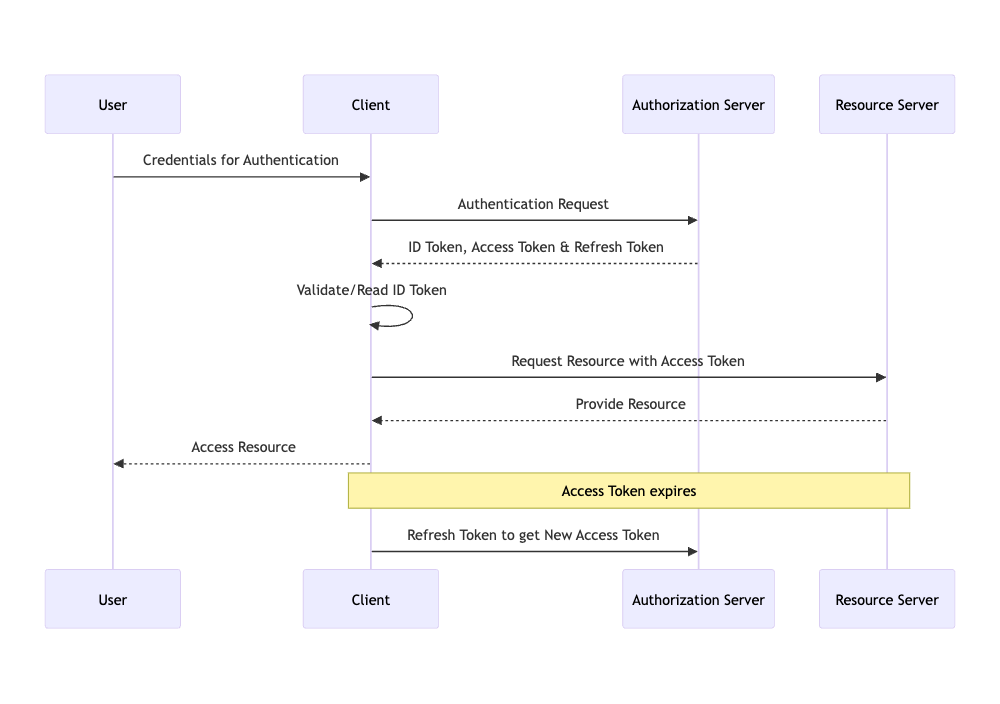
\includegraphics[width=\textwidth, height=320px]{pics/implicit_flow.png}
\end{figure}

\chapter{Threat Modelling}
\label{chap:threat_model}
Threat modelling is an act of security analysis which aids in discovering potential vulnerabilities in an application or a system before they become threats \citep{threat_model_intro}.
This exercise is a crucial step in the Software Development Life Cycle (SDLC), as it helps detect the possible flaws in the system, and suitable mitigation can be applied.
Therefore, we conduct threat modelling for a scenario, where an authentication server using OIDC protocol is operated in a cloud environment.
We favor Shostack's Four Question Framework \citep{shostack} to guide the threat modelling in this work.
The questions focus on the project objectives, namely what could go wrong, what mitigations are appropriate and what can be improved.
Using Shostacks questions in conjunction with the OWASP threat modelling process, the application can be analysed using OIDC in the cloud \citep{owasp_threat_model}.
The objective of threat modelling is to identify as many possible risks present in the Open ID Connect application running on a cloud.
Furthermore, the modelling is cloud agnostic, meaning these identified mitigations can be applied anywhere, irrespective of the cloud provider.

\section{Application Information}
To answer the first question from Shostacks's Four questions, \textit{what are we working on}, this section describes the application and the different dependencies that this application contains.
\newpage
\begin{itemize}
    \item \textbf{Application Name:} Multi-tenant App
    \item \textbf{Application Version:} v1.0
    \item \textbf{Description:} This generic authentication and authorisation application utilises OIDC protocols PKCE flow (refer to Figure \ref{fig:pkce_flow}) in a public cloud environment.
    This application is based on multi-tenant capability, where the users cannot access each other's resources even though they share the same infrastructure and application.
    This general API would provide the capabilities mentioned in Table \ref{table:threat_model_entry_points}.
  \end{itemize}

\subsection{Entry Points}
\begin{longtable}{|p{3cm}|p{4cm}|p{4cm}|p{4cm}|}
\caption{Entry Points for the prototype}
\label{table:threat_model_entry_points}
\hline
\rowcolor{grey!15}
\textbf{Entry Point} & \textbf{Description} & \textbf{Request Parameters} & \textbf{Response Data} \\
\hline
\endfirsthead
\hline
\rowcolor{grey!15}
\textbf{Entry Point} & \textbf{Description} & \textbf{Request Parameters} & \textbf{Response Data} \\
\hline
\endhead
\endfoot
\hline
\endlastfoot

/authorize & Entry point for user authentication by the Authorisation server.  & 
- \textit{client\_id}: The client ID of the application \newline 
- \textit{redirect\_uri}: URI where the response will be sent \newline
- \textit{scope}: Scopes for requested authentication (e.g., OpenID, email) \newline 
- \textit{response\_type}: Indicates the desired authorisation flow (e.g., code) \citep{openid_docs} & 
- The authorisation code is to be exchanged for tokens. \newline 
- Error in case of invalid request \\
\hline

/token & Entry point for exchanging authorisation code for tokens (access token, ID token, refresh token). & 
- \textit{grant\_type}: "authorization\_code" \newline 
- \textit{code}: Authorisation code received from /authorize \newline
- \textit{redirect\_uri}: Must match the original redirect URI used in /login \newline 
- \textit{client\_id}: The client ID of the application
- \textit{code\_verifier}: Code used to validate code\_challenge \citep{openid_docs}& 
- \textit{access\_token}: Token for accessing protected resources \newline 
- \textit{id\_token}: Token containing user identity information \newline 
- Error in case of invalid request \\
\hline

\end{longtable}

\begin{longtable}{|p{8cm}|p{8cm}|}
\caption{Asset Descriptions}
\label{table:threat_model_assets}
\hline
\rowcolor{grey!15}
\textbf{Assets} & \textbf{Description} \\
\hline
\endfirsthead

\hline
\rowcolor{grey!15}
\textbf{Assets} & \textbf{Description} \\
\hline
\endhead

% Assets for PKCE App in Cloud with Multiple Tenants
OAuth Tokens & Used to authorise access to resources on behalf of the user. \\
\hline
User Credentials & Sensitive information (e.g., usernames, passwords) used to authenticate users; protection. \\
\hline
OAuth Authorisation Codes & Temporary codes exchanged during OAuth flows are essential for secure authorisation in PKCE flows. \\
\hline
Cloud Infrastructure & The underlying infrastructure (servers, storage, networking) that supports the application in the cloud \\
\hline
Application Data & Data created, stored, or processed by the application, which could include user data or system configurations \\
\hline
API Endpoints & Points of interaction where the application exposes functionality to clients (Refer to Table \ref{table:threat_model_entry_points}, to see the entry-points). \\
\hline

\end{longtable}


\section{STRIDE Model}
Using the given entry points and assets that the application uses, a level zero Data Flow Diagram (refer to Figure \ref{fig:dfd_app_fig}) is created.
This diagram provides an overview of the system's significant processes, data flow, and credential stores.
This abstraction of the system proceses can be explicitly used for threat modelling, e.g., STRIDE \citep{dfd_stride}.
STRIDE is a threat modelling framework used to classify security threats developed by Microsoft \citep{stride_usage}.
The letters in the acronym are Spoofing, Tampering, Repudiation, Information Disclosure, Denial of Service, and Elevation of Privilege.
The threat categories are analysed during the threat modelling \citep{stride}.
Using the DFD, a STRIDE threat modelling is carried out, which provides an analysis of some threats in the given context of this model.
This threat modelling framework is chosen because it allows for a systematic and structured approach to identify threats in different areas denoted by the acronym and is easy to apply.



\begin{figure}[h!]
\centering
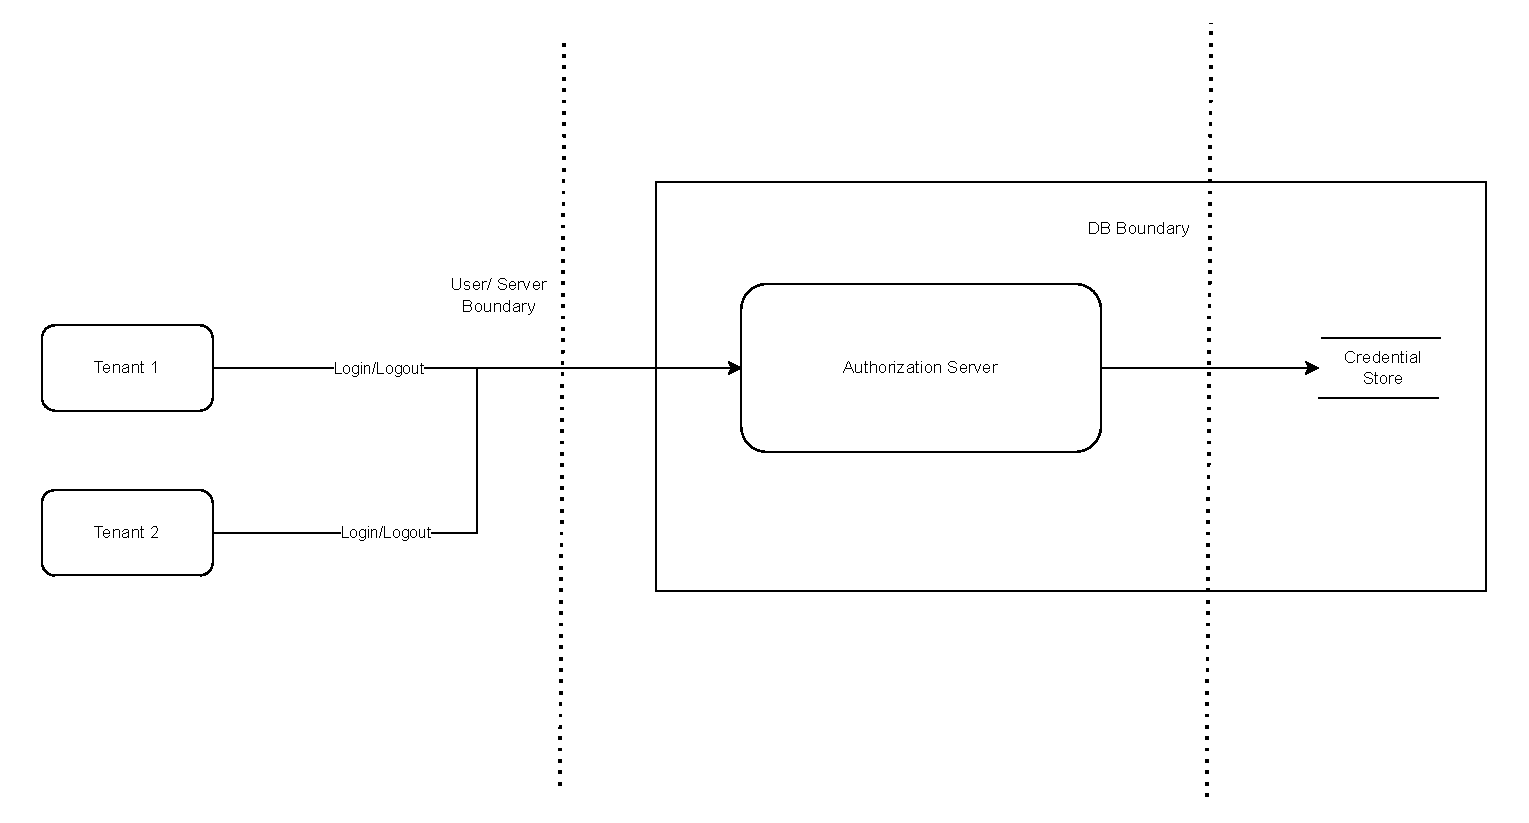
\includegraphics[width=\textwidth]{pics/DFD_APP.pdf}
\caption{Data Flow Diagram Level 0 OIDC App}
\label{fig:dfd_app_fig}
\end{figure}


\label{subsec:stride}
\subsection*{1. Spoofing}
\begin{itemize}
    \item \textbf{Threat}: An attacker attempts to impersonate a legitimate user or tenant to gain unauthorised access.
    \item \textbf{Specific Attacks}:
    \begin{itemize}
        \item \textbf{ID Spoofing}: The attacker tries impersonating an end user from another OpenID Provider by using spoofed tokens or changing the token's contents \citep{oidc_attacks}.
        \item \textbf{Credential Stuffing}: Using leaked credentials from other services to gain unauthorised access.
        \item \textbf{Phishing}: Tricking users into providing their credentials through fraudulent login pages. For example, the attackers can manipulate the redirect endpoints to redirect to the malicious URL \citep{open_redirect_oidc_threat}.
        \item \textbf{Man-in-the-Middle Attack (MITM)}: Intercepting the authorisation code during the OAuth2 flow.
    \end{itemize}
    \item \textbf{Mitigation}:
    \begin{itemize}
        \item Signed tokens should always be verified at the issuer's end so that a spoofed token cannot bypass the security.
        \item The client should validate the audience and issuer claims to prevent tokens from being used across different services.
        \item Enforce multi-factor authentication (MFA) to prevent credential-based attacks.
        \item PKCE mitigates MITM attacks by tying the authorisation code to a unique challenge/response.
        \item Use OAuth2’s \texttt{nonce} and \texttt{state} parameters to protect against replay attacks.
    \end{itemize}
\end{itemize}

\subsection*{2. Tampering}
\begin{itemize}
    \item \textbf{Threat}: Unauthorised modification of data or code during transmission or at rest.
    \item \textbf{Specific Attacks}:
    \begin{itemize}
        \item \textbf{Token Tampering}: This attack targets access, ID, and refresh tokens. Where the attacker manipulates the tokens to add their claims and scopes to allow authorised access \citep{oidc_attacks}.
        \item \textbf{Code Injection}: Injecting malicious code or tokens into the OAuth2 flow.
        \item \textbf{OAuth Token Replay}: Reusing an old token after invalidating or expired.
        \item \textbf{Malicious Endpoint} The discovery endpoints of OIDC, such as the ./wellknown, are tampered with, and malicious endpoints are added to the public endpoint where the attacker can now get sensitive information, as the endpoints are fake \citep{oidc_attacks}.
        \item \textbf{Ransomware}: Unlike just OIDC, cloud technologies, especially public clouds, are susceptible to ransomware attacks. In this attack, the attacker tries to misuse existing vulnerabilities and steal sensitive data or encrypt it, making it unusable \citep{ransomeware}.
    \end{itemize}
    \item \textbf{Mitigation}:
    \begin{itemize}
         \item A key should always sign the tokens like ID tokens containing user information and must be verified each time with the issuer when used.
        \item Use PKCE to prevent authorisation code injection by requiring a code challenge.
        \item Sign and validate JWT tokens to ensure integrity and detect tampering.
        \item Implement token expiration and invalidation mechanisms and rotating refresh tokens to reduce token reuse.
        \item Use different tools like SIEM to detect anomalies in the system and prevent malware such as ransomware from propagating deep into different services into the cloud \citep{ransomeware}.
        \item Perform network segregation and build zero privilege systems to allow only the required actors to access the services and no more \citep{zero_trust}. 
    \end{itemize}
\end{itemize}

\subsection*{3. Repudiation}
\begin{itemize}
    \item \textbf{Threat}: Users or tenants could deny performing certain actions, making it difficult to establish accountability.
    \item \textbf{Specific Attacks}:
    \begin{itemize}
        \item \textbf{Action Denial}: A malicious tenant denies having issued a token or performed an action within the application that could deny sending or receiving messages in a digital transaction \citep{repudiation}.
        \item \textbf{Tenant Switching}: Similarly, in a multi-tenant environment, a user might gain access to another tenant’s data and deny the action.
    \end{itemize}
    \item \textbf{Mitigation}:
    \begin{itemize}
        \item Use signed access tokens (JWT) with non-repudiation attributes.
        \item Log every critical action and tenant interaction, including token issuance and API calls, with cryptographically signed entries.
        \item Use immutable logs with encryption.
    \end{itemize}
\end{itemize}

\subsection*{4. Information Disclosure}
\begin{itemize}
    \item \textbf{Threat}: Sensitive data such as access tokens, personal data, or tenant-specific information is exposed.
    \item \textbf{Specific Attacks}:
    \begin{itemize}
        \item \textbf{Cross-Tenant Data Leakage}: Improper multi-tenant isolation could make one tenant’s data accessible to another.
        \item \textbf{Token Exposure}: OAuth2 tokens might be leaked through insecure communication.
        \item \textbf{Cloud Misconfigurations}: Misconfigured database leading to data exposure.
    \end{itemize}
    \item \textbf{Mitigation}:
    \begin{itemize}
        \item Implement strong tenant isolation at the application and database levels, ensuring no cross-tenant data leakage.
        \item Use end-to-end encryption and enforce HTTPS for all communications.
        \item Conduct regular security audits to identify cloud misconfigurations.
        \item Manage whitelisted redirect URIs and limit callback URLs to trusted domains.
        \item Use automated tools to scan for and fix misconfigurations like OWASP Zap \citep{owasp_zap}.
    \end{itemize}
\end{itemize}

\subsection*{5. Denial of Service (DoS)}
\begin{itemize}
    \item \textbf{Threat}: An attacker may overwhelm the service, making it unavailable for legitimate users and tenants.
    \item \textbf{Specific Attacks}:
    \begin{itemize}
        \item \textbf{Token Bombing}: Repeatedly requesting tokens using valid credentials to overload the authorisation server.
        \item \textbf{API Rate Limiting Attack}: Flooding API endpoints with excessive requests, leading to resource exhaustion.
        \item \textbf{Resource Starvation}: Exploiting vulnerabilities to consume cloud resources, like CPU or memory, disrupting multi-tenant services.
    \end{itemize}
    \item \textbf{Mitigation}:
    \begin{itemize}
        \item Implement API rate limiting and token request throttling to prevent a token bombing.
        \item Use distributed denial of service (DDoS) protection services, such as AWS Shield \citep{aws_shield}.
        \item Ensure each tenant has isolated resource pools to avoid one tenant's traffic affecting others.
        \item Implement service quotas for resource consumption per tenant.
    \end{itemize}
\end{itemize}

\subsection*{6. Elevation of Privilege}
\begin{itemize}
    \item \textbf{Threat}: An attacker could gain higher privileges than authorised, allowing access to sensitive data or functionality.
    \item \textbf{Specific Attacks}:
    \begin{itemize}
        \item \textbf{PKCE Downgrade Attack}: The attacker can remove \texttt{code\_challenge} from the request if the authentication server does not validate the \texttt{code\_verifier}, the token will be issued, allowing unauthorised access \citep{oidc_attacks}.
        \item \textbf{Insecure Multi-Tenant Access Control}: A user accessing other tenants' resources through misconfigured roles or policies.
    \end{itemize}
    \item \textbf{Mitigation}:
    \begin{itemize}
        \item The \texttt{code\_verifier} must be verified at the authentication server and the \texttt{code\_challenge} should be bound the the authorisation code \citep{oidc_attacks}.
        \item Regularly audit role assignments, permissions, and token scopes to detect misconfigurations.
        \item Implement tenant-aware access control to ensure that users can only interact with resources belonging to their tenant.
    \end{itemize}
\end{itemize}


\section{Risk Assessment}
Risk assessment is integral to keeping a system safe as it helps identify, analyse and evaluate the potential risks that could negatively impact an organisation. Cyber breaches have an enormous impact on an organisations value and reputation; for example, in 2024 \citep{ibm} estimated the average cost of a cyberattack on a company in the US is about 4.88M USD. In addition, such data breaches also could cost firms penalties due to non-compliance, especially in the EU. Organisations face hefty fines of up to 10 Million Euros or 2\% of their worldwide revenue under GDPR Article 83 \citep{gdpr_fine}. Therefore, carrying out a risk assessment helps understand the impact of these risks and determine how to manage and address the potential issues before they occur. 

In the cybersecurity space, there are several well-known risk assessment frameworks like Factor Analysis of Information Risk [FAIR], Operationally Critical Threat Asset and Vulnerability Evaluation [OCTAVE], NIST Cybersecurity Framework, and ISO/IEC 27001 \citep{cybersec_risk_frameworks}. Each of these frameworks has its strengths and weaknesses; for example, FAIR considers the frequency of attacks and provides valuable information regarding financial losses \citep{fair_bn}, and OCTAVE and NIST also have their advantages. However, the framework ISO/IEC 27001:2022 is chosen for this project, as this standard focuses exclusively on information security risk management and offers guidance on identifying, accessing, and information systems \citep{iso}. Choosing ISO 27001:2022 provides a significant advantage in its alignment with the ISO/IEC 27000 family, a recognized standard for establishing an Information Security Management System (ISMS). In addition to its compatibility with ISO 27001:2013, this assessment method provides flexibility in adapting to different industries and their sizes. \cite{iso_2700:2022} also states that ISO/IEC 27001:2022 slightly improved to ISO/IEC 27001:2013, consisting of additional protection to cloud computing services, which is also being analysed in this assessment. Following this framework, the following sections will define the scope, methodology, limitations, analysis, and non-compliance risks following local laws like GDPR. 


\subsection{Scope}
The first step in this risk assessment process is to define the scope of the ISMS, as it plays a crucial role in identifying, analyzing, and evaluating the risk effectively. Using the scopes, one can limit the analysis to a particular subject and focus on the priorities. The scope is constrained to a small prototype implementing a multi-tenant authentication application using PKCE flow in a cloud application, which resembles a small business. The IT assets are listed in Table \ref{table:threat_model_assets}, and the physical usage of this application is located in the European Union, meaning the regulatory measures that need to be followed are based in this region, especially GDPR. The key elements that are part of the scope are as follows:
\begin{itemize}
    \item Cloud Security
    \item Multi-tenancy Issues
    \item PKCE Implementation Issues
    \item Data Security and Privacy
    \item Regulatory and Compliance Requirements
    \item Identity and Access Management (IAM)
\end{itemize}

\subsection{Methodology}
One of the benefits of using risk assessment from the ISO/IEC 27000 group is that it does not prescribe a specific methodology for quantitative or qualitative analysis. In contrast to FAIR, which is a quantitative method, qualitative, quantitative, or a mix of both can be applied here. 

The assessment of this project is based on qualitative analysis rather than quantitative analysis due to the complexity and nature of the risks. For instance, risks identified during threat modelling, such as data isolation, cloud misconfiguration, and shared resource vulnerabilities, are difficult to quantify because they involve unknown factors. Using subjective analysis simplifies the decision-making process and is faster to conduct. To assess the risks meaningfully, the Common Attack Pattern Enumeration and Classification (CAPEC) is used as a reference. CAPEC provides a comprehensive database for the technical exploits used by adversaries and focuses on application security. CAPEC categorizes the general likelihood and severity into five levels, ranging from very low to very high. These levels are then converted to a number from 1-5 for each to determine the risk level for a specific threat (CAPEC). Figure \ref{fig:ris_assessment_method} depicts the process of ranking severity and liklihood, using CAPEC and create a risk matrix as a structured report of threats and their risk level. 

\begin{figure}[h!]
\centering
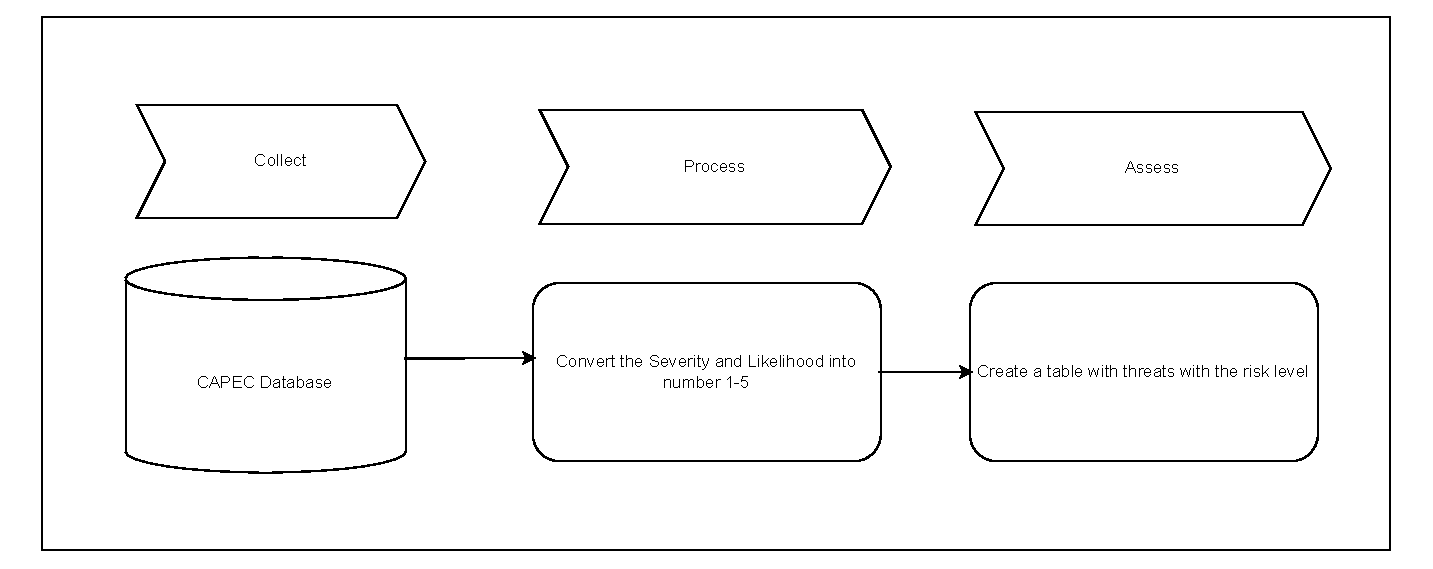
\includegraphics[width=\textwidth]{pics/risk_assessment_method.pdf}
\caption{Rank the severity and likelihood using a qualitative scale (1-5)}\label{fig:ris_assessment_method}
\end{figure}

\newpage
\textbf{Definitions}:
    \begin{itemize}
        \item  \textbf{Likelihood (1-5)}: Likelihood of the attack happening based on the current environment, known vulnerabilities, and ease of exploitation.          \begin{itemize}
            \item \textbf{1}: Very unlikely
            \item \textbf{5}: Very likely
         \end{itemize}
        \item \textbf{Impact (1-5)}: Impact of the attack on the system, focusing on data breaches, financial loss, service downtime, and customer trust.
         \begin{itemize}
            \item \textbf{1}: Very Low
            \item \textbf{5}: Very High
         \end{itemize}
         
       \item  \textbf{Risk Level (1-25)}: Calculated as Likelihood × Impact. High values indicate higher overall risk. 
       \begin{itemize}
           \item \textbf{1-5}: Very Low Risk = Requires minimal attention.
           \item \textbf{5-10}: Low Risk = Requires minimal attention.
           \item \textbf{10-15}: Medium Risk = Needs monitoring and potentially preventive measures.
           \item \textbf{15-20}: High Risk = Immediate action required to mitigate the risk.
           \item \textbf{20-25}: Very High Risk = Immediate action required to mitigate the risk.

       \end{itemize}
    \end{itemize}

    
\subsection{Limitations}  
Although ISO/IEC 20071:2022 is an internationally recognized standard for risk assessment, the framework and scope of this project have some limitations which we list below in regards to our methodology:

\begin{itemize}
    \item The complexity of full implementation requires assessing organisational, human, physical, and technological controls as per ISO/IEC 20071:2022. However, since this is merely a prototype, only technological controls are being considered, limiting this framework's effectiveness.
    
    \item The data used from CAPEC to derive the likelihood and impact is a generic value and can differ from the actual case, which could cause some deviation from the analysis.
    
    \item Some attacks are not listed in the CAPEC database, which then is assessed subjectively according to their complexity and impact. 
    
    \item Given the timeframe of this project and the limited resources, not all aspects of this framework can be implemented and documented. Instead, only the scope, methodology, and risk assessment.
    
    \item It is very resource intensive, and the assessment result is based on a specialist doing the analysis, which could lead to subjective arguments.
    
    \item The project's scope is narrow, mainly focusing on the technical risks of this implementation. This could leave some specific systems not being covered. For example, the amount of financial loss that would occur with different risks is not covered.

\end{itemize}

\subsection{Qualitative Analysis of Risks}
 This section is core to the contributions of this work and forms the backbone of the research findings.
 It consists of data on the threats that affect the OIDC application in a cloud environment.
 Several research papers, journals and theses studied in this work form the basis of the qualitative assessment of each threat.
 To answer the research question (refer to Section \ref{sec:objectives}) mentioned in Chapter 1, the different technical threats and risks that occur due to non-compliance to regulations are analysed.
 As the methodology mentions, the collected threats are compared against the CAPEC database and are qualitatively assessed.
 Table \ref{table:risk_assessment} shows the threats quantified, and the risk level is ordered from highest to lowest. 

\definecolor{ForestGreen}{rgb}{0.13, 0.55, 0.13}

\begin{longtable}{|>{\raggedright}p{4cm}|>{\centering\arraybackslash}p{2cm}|>{\centering\arraybackslash}p{2cm}|>{\centering\arraybackslash}p{2cm}|>{\centering\arraybackslash}p{3cm}|}
\caption{Table: Risk Assessment}
\label{table:risk_assessment}
\hline
\rowcolor{grey!15}
\textbf{Threat} & \textbf{Likelihood (1-5)} & \textbf{Impact (1-5)} & \textbf{Risk Level (1-25)} & \textbf{CAPEC ID}\\
\hline
\endfirsthead

\hline
\rowcolor{grey!15}
\textbf{Threat} & \textbf{Likelihood (1-5)} & \textbf{Impact (1-5)} & \textbf{Risk Level (1-25)} & \textbf{CAPEC ID}\\
\hline
\endhead

\hline
\endfoot

\hline
\endlastfoot
Cloud Misconfigurations & 4 & 5 & \cellcolor{red!90} 20 & - \\
\hline
Phishing & 4 & 5 & \cellcolor{red!90} 20 & CAPEC-98  \\
\hline
MitM & 4 & 5 & \cellcolor{red!90} 20 &  CAPEC-94\\
\hline
Credential Stuffing & 4 & 4 & \cellcolor{red!60} 16 & CAPEC-600 \\
\hline
Code Injection (XSS, SQLi) & 4 & 4 & \cellcolor{red!60} 16 & CAPEC-242 \\
\hline
Token Tampering & 4 & 3 &  \cellcolor{yellow!90} 12 &CAPEC-39 \\
\hline
Ransomware & 3 & 4 &  \cellcolor{yellow!90} 12 & CAPEC-549 \\
\hline
Insecure Multi-Tenant Access Control & 3 & 4 &  \cellcolor{yellow!90} 12 & - \\
\hline
Action Denial (Denial of Service) & 4 & 3 &  \cellcolor{yellow!90} 12 & CAPEC-125\\
\hline
ID Spoofing & 3 & 3 &  \cellcolor{green!20} 9 & CAPEC-151\\
\hline

PKCE Downgrade Attack & 2 & 4 & \cellcolor{green!20} 8 & -\\
\hline
Cross-tenant data Leakage & 1 & 4 &  \cellcolor{ForestGreen} 4 & CAPEC-546 \\
\hline

\end{longtable}
 \noindent In total, 12 threats are analysed and ranked according to their risk level.
 Figure \ref{fig:Risk Level Counts} depicts a bar chart showing the risk level distribution of the analysed threats.
 This analysis identifies three very high, two high, four moderate, two low and one very low risk.
 The mitigations for these threats have already been mentioned in Sub-Section \ref{subsec:stride}; however, this section highlights the level of risk each threat poses to an organisation.
 The high and high risks must be mitigated before the application is published. 

\begin{figure}[h!]
\centering
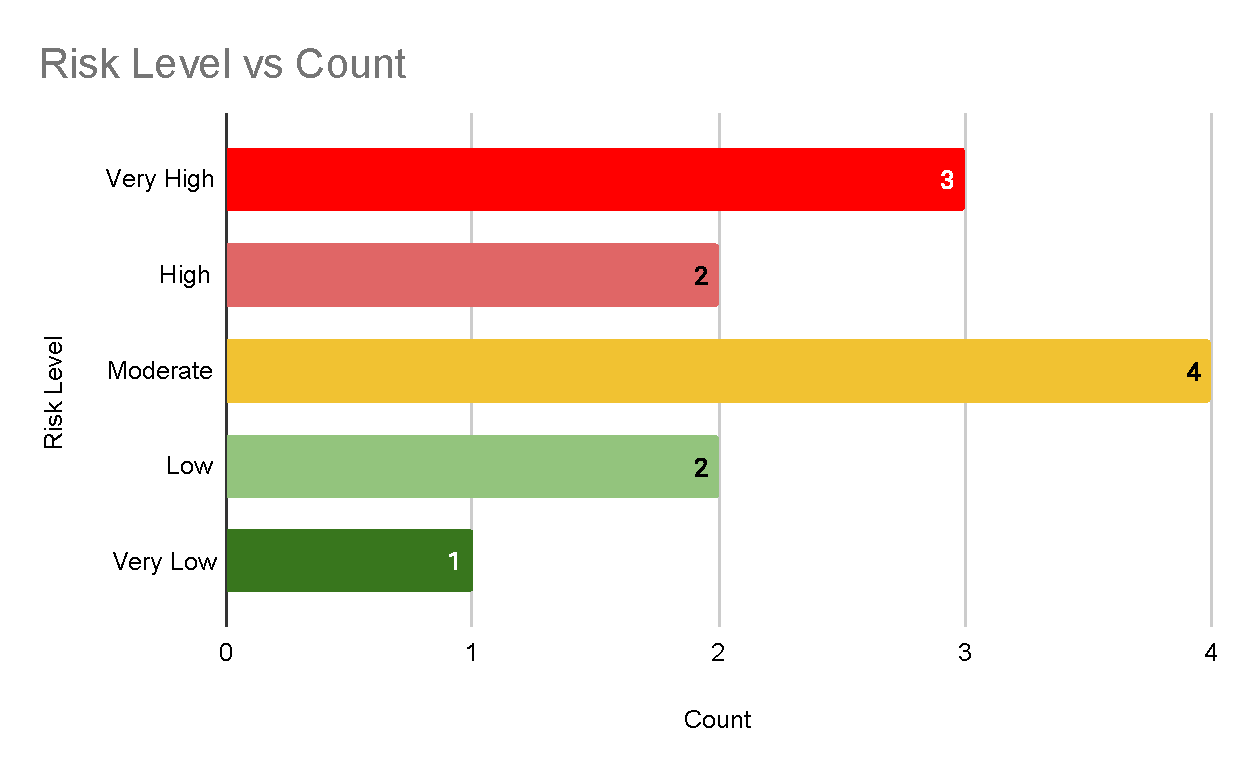
\includegraphics[width=\textwidth]{pics/risk_level_vs_count.pdf}
\caption{Distribution of Risk levels}\label{fig:Risk Level Counts}
\end{figure}

\subsection{Non-Compliance Risk}
Non-compliance is a failure to adhere to established laws, regulations, and standards, especially in today's digital age, where vast amounts of sensitive data are also called personally identifiable information (PII). Such personal data are stored, processed, and transferred among different firms. Therefore, protecting private data is a significant priority; hence, various laws and rules bind companies and organisations to protect sensitive data. One of the most stringent data protection frameworks globally is the GDPR act, concerned with data processing of EU residents \citep{gdpr_stringent}. 

Operating an OIDC application in the cloud carries a high risk if it does not comply with GDPR laws. OIDC involves handling personal data, such as user information, so ensuring compliance with GDPR is crucial when working with such an application. To avoid the risk of non-compliance with GDPR, potential financial loss, and damage to reputation, specific key mitigations need to be implemented before publishing the applications. The following are the key provisions from \citep{gdpr_law} that present potential risks according to the GDPR law:


\begin{itemize}
    \label{section:gdpr}
    \item \textbf{Article 6 GDPR}: There should be a lawful basis for processing personal data to fulfil a contractual obligation for the data controller. Organisations must document the lawful basis for processing personal data and ensure transparency in informing users about why their data is being processed. In addition, this article also states the requirement of consent with concise text without vague legal jargon and the functionality to withdraw consent.
    
    \item \textbf{Articles 15-22 GDPR}: "Data subject rights": proper access, rectification, erasure, and portability. These rights should be able to exercised by the users. 

    \item \textbf{Article 25 GDPR}: "Data Protection by Design and by Default": This article requires organisations to embed safeguards into their systems and processes, such as data minimization and encryption, are integrated into system development, reducing risks proactively and ensuring privacy. 

    \item \textbf{Article 32 GDPR }: Appropriate Security measures must be taken to protect sensitive data, such as encrypting data, maintaining access control lists, regular audits, and security checks. Failure to implement these measures can result in security breaches, leading to unauthorised access to personal data and violations of GDPR’s security requirements.
    
    
    \item \textbf{Chapter V GDPR }: Cloud based applications often operate across borders. This makes it more important to consider where sensitive data such as PII are stored. GDPR imposes strict rules on transferring personal data to countries outside the European Economic Area (EEA) unless those countries have been deemed to provide adequate data protection. This chapter of GDPR stipulates that providers that are also located outside the EEA must be compliant with GDPR rules. As popular cloud providers such as AWS, Google, and Microsoft operate outside the EEA, this law plays a big role with cloud providers.  
.
\end{itemize}

\section{Conclusion}

Conducting a thorough risk assessment for an OIDC application deployed in the cloud is crucial to identify potential security vulnerabilities and ensure GDPR compliance. OIDC applications handle sensitive personal data during user authentication and authorisation, making them susceptible to threats such as cloud misconfigurations, phishing, MitM attacks, token tampering, and cross-tenant data leakage. These threats can significantly impact personal data's confidentiality, integrity, and availability. 

Therefore, using the threat modelling results, we identified the threats and their mitigations, and the qualitative risk analysis helped us rank these threats according to their risk level. By prioritizing threats based on their perceived risk, we can increase efficiency. In addition to the threats, not complying with GDPR will result in significant financial costs for the organisation, making it a high-risk factor. As a result, high-risk threat mitigations must be applied to GDPR measures to ensure regulatory adherence. 









\chapter{Design}

In Chapter \ref{chap:threat_model}, we discussed the threat modelling of an OpenID Connect application implemented using PKCE on a cloud environment. The threat modelling provided an in-depth understanding of potential attack vectors and risks that could compromise the cloud-based application using the OpenID Connect Protocol. Building upon the insights gathered from the threat modelling exercise (See \ref{subsec:stride}), this chapter will focus on the design of a prototype that would address some of the threats identified. We will describe the implementation decisions and design choices made to mitigate identified risks and establish a secure, scalable, and efficient cloud-based authentication system using PKCE on AWS.


\section{Limitations}
\chapter{Results and Discussions}

This chapter presents a comprehensive evaluation and validation of the security implementation mechanisms detailed in Section \ref{sec:sec_impl}. We systematically examine multiple security aspects through various testing procedures, including evaluating authentication mechanisms, conducting OIDC PKCE compliance tests, identifying cloud vulnerabilities, performing password hash compare timing tests, and assessing access control mechanisms. The investigation meticulously documents and analyses the empirical results, revealing the strengths and potential vulnerabilities of the implemented security framework.


\section{Manual Testing}
As a pre-condition for testing the two PKCE endpoints, a build script (refer to Appendix \ref{apendix:build_and_run_script}) is executed. This build script creates the required infrastructure by running the terraform, like the lambdas and API gateways. In addition to providing the infrastructure, the database will be seeded with two tenants and some users. In this section, manual tests of the two endpoints implemented are documented.


\subsection{Authorise Endpoint}
Manual tests were conducted on the \textbf{/authorize} endpoint to assess its functionality and security measures. The testing process included the following scenarios:

\begin{enumerate}
     \item \textbf{Successful Authentication:} Verified that the endpoint correctly processes authentication requests when provided with valid credentials, a valid client ID, and a proper code challenge. Additionally, the test was repeated successfully using \textbf{Tenant 2} to ensure multi-tenant compatibility. Figure \ref{fig:authorize_tenant_1_success} shows the successful authentication of a user in \textit{tenant 1} when all the required parameters and the credentials are correct, and Figure \ref{fig:authorize_tenant_1_wrong_pass} presents a successful authentication with \textit{tenant 2}.

\begin{figure}[!htbp]
    \centering
    \begin{lstlisting}[style=curlstyle]
Request:
curl -X POST http://tenant1.local:4566/restapis/o4qbjcrrti/dev/_user_request_/
authorize\
-H "Content-Type: application/json" \
-d '{"username": "user7@example.com","client_id":"tenant1-client-id-1", "password": "test1"}'

Response:{
"message":"Hello, user7@example.com",
"authorizationCode":{"S":"22f51d86-c29b-49ef-a594-9916d10a7617"},
"expiresAt":{"N":"1734690017"}
}
    \end{lstlisting}
    \caption{Successful user Authorise for tenant1}
    \label{fig:authorize_tenant_1_success}
\end{figure}


\begin{figure}[!htbp]
    \centering
    \begin{lstlisting}[style=curlstyle]
Request:
curl -X POST http://tenant2.local:4566/restapis/o4qbjcrrti/dev/_user_request_/authorize \                                  
-H "Content-Type: application/json" \
-d '{"username": "user7@example.com","client_id":"tenant2-client-id-1", "password": "test2", "codeChallenge": "ChX9V18izIUew6V7-DRS4hMRK3H_tlPBQ5E_umRHLNo"}'

Response:{
"message":"Hello, user7@example.com",
"authorizationCode":{"S":"79641e2f-2a32-46ef-9e61-263ba620acff"},
"expiresAt":{"N":"1734693110"}
}
    \end{lstlisting}
    \caption{Successful user Authorise for tenant2}
    \label{fig:authorize_tenant_2_success}
\end{figure}

\newpage
    \item \textbf{Authentication Failures:} Tested various failure scenarios to ensure the system handles them securely and as expected:
    \label{subsec:auth_failure_tests}
    \begin{itemize}
        \item \textbf{Invalid Credentials:} Attempted authentication with incorrect tenant credentials to confirm that the system denies access and provides appropriate error responses. Figure \ref{fig:authorize_tenant_1_wrong_pass} illustrates the denial of access that occurs when a user provides a wrong password.

        \begin{figure}[!htbp]
    \centering
    \begin{lstlisting}[style=curlstyle]
Request:
curl -X POST http://tenant2.local:4566/restapis/o4qbjcrrti/dev/_user_request_/authorize \                                  
-H "Content-Type: application/json" \
-d '{"username": "user7@example.com","client_id":"tenant2-client-id-1", "password": "wrong_password", "codeChallenge": "ChX9V18izIUew6V7-DRS4hMRK3H_tlPBQ5E_umRHLNo"}'

Response:{
"message":"Invalid username or password"}
}
    \end{lstlisting}
    \caption{Unsuccessful user Authorise for tenant1 with wrong password}
    \label{fig:authorize_tenant_1_wrong_pass}
\end{figure}

        

       
        \item \textbf{Unknown Client ID:} Tested requests with an unregistered or invalid client ID to confirm the endpoint rejects such requests without further processing. Figure \ref{fig:authorize_tenant_1_unknown_client} depicts the curl request with \textit{tenant 1}
        and an unknown \textit{client\_id}, and responds with access deined with a corresponding error message.

\begin{figure}[!htbp]
    \centering
    \begin{lstlisting}[style=curlstyle]
Request:
curl -X POST http://tenant1.local:4566/restapis/o4qbjcrrti/dev/_user_request_/authorize \                                  
-H "Content-Type: application/json" \
-d '{"username": "user7@example.com","client_id":"unknown-client-id-1", "password": "test2", "codeChallenge": "ChX9V18izIUew6V7-DRS4hMRK3H_tlPBQ5E_umRHLNo"}'

Response: {"message":"Invalid client ID"}
    \end{lstlisting}
    \caption{Unsuccessful user Authorise for tenant1 with Unknown Client}
    \label{fig:authorize_tenant_1_unknown_client}
\end{figure}


    \end{itemize}
\end{enumerate}

These tests helped validate the robustness of the \textbf{/authorize} endpoint, ensuring it functions correctly under normal conditions while effectively mitigating common security threats.

\newpage
\subsection{Token Endpoint}
Manual tests were also conducted on the \textbf{/token} endpoint to verify its functionality and robustness. The following scenarios were tested:

\begin{enumerate}
    \item \textbf{Successful Token Retrieval:} Verified that the endpoint successfully issues tokens when provided with a valid authorisation code, client ID, and code verifier. The tokens are signed using an asymmetric key using the RS256 Algorithm (Refer to Figure \ref{fig:token_tenant_1_token_signed}). The private key is generated using the RSA-2048-bit algorithm (refer to Appendix \ref{apendix:create_private_keys}), and the keys are stored securely in the secrets manager, which the token lambda retrieves (Refer to Appendix \ref{apendix:token_signing}). Figure \ref{fig:token_tenant_1_success} illustrates a successful retrieval of an access token of a user after authentication.


        \begin{figure}[!htbp]
    \centering
    \begin{lstlisting}[style=curlstyle]
Request:
curl -X POST http://tenant1.local:4566/restapis/o4qbjcrrti/dev/_user_request_/token\                                      
-H "Content-Type: application/json" \
-d '{
    "username": "user7@example.com","grant_type": "authorization_code","client_id":"tenant1-client-id-1", "authorizationCode": "a24e5543-7ed6-4511-a021-be911004f187", "codeVerifier": "wOV-nI-            
    QSyesPpyjPpyjkBPx7PCimGUBrxOqKgc8idU
    NLnzeIkUq1nJI4R2hEyoolgexTqQfAd4hbX8mi
    7ud0BpQv16u6R9a14fWjXjj65uWDnV-nfI7Ow-YaippAChI
"}'

Response: {
    "token":"eyJhbGciOiJSUzI1NiIsInR5cCI6IkpXVC
    J9.eyJ1c2VySWQiOiJ1c2VyLTI2Mjc3LTEyMjc2IiwiaWF0
    IjoxNzM0NzAwNDg5LCJleHAiOjE3MzQ3MDQwODl9.NMjBNY
    w4rprZ_irSFv0MKWrIt3KiOtteNeDDvwlv-T2QMpcgIEfdT5
    Nvc_zjIOotayqiHHtQNBQf_j-Y89z52Sv-076UaQOq5SeEU52
    voaqUABAQ5QoaaTELmCWMDOovAK9_9fo
    sF0Am5hMYBZe3S8H0vUKqdSM1Bcu2ONAo40tRCowfK90NHp1q5A
    2CBuXanbCiVYrzZZ0Bes6y0Xpun6ldu8FnSIzgmzE3sPCGmmRP5E
    kE1IoW2ViQ4irklUkFWXBZDjoZZua9CoPzcgH0OWD_uL48ZqSiXO
    PbvO_TcKCZ5ORnHPdeN7PRupllUFaR-M9B4yZtfjujFBHBSi63A"
}
    \end{lstlisting}
    \caption{Successful token retrieval for tenant 1}
    \label{fig:token_tenant_1_success}
\end{figure}

\newpage
    \item \textbf{Expired Authorisation Code:} Attempted to retrieve a token using an expired authorisation code to ensure the endpoint denies the request with an appropriate error response. Figure \ref{fig:token_auth_code_expired} illustrates the denial of authority when the token endpoint is requested with an expired user \texttt{authorisation code}.
    
    
    \begin{figure}[!htbp]
    \centering
    \begin{lstlisting}[style=curlstyle]
Request:
curl -X POST http://tenant1.local:4566/restapis/o4qbjcrrti/dev/_user_request_/token\                                      
-H "Content-Type: application/json" \
-d '{
    "username": "user7@example.com","grant_type": "authorization_code","client_id":"tenant1-client-id-1", "authorizationCode": "a24e5543-7ed6-4511-a021-be911004f187", "codeVerifier": "wOV-nI-            
    QSyesPpyjPpyjkBPx7PCimGUBrxOqKgc8idU
    NLnzeIkUq1nJI4R2hEyoolgexTqQfAd4hbX8mi
    7ud0BpQv16u6R9a14fWjXjj65uWDnV-nfI7Ow-YaippAChI
"}'

Response: {"message":"Invalid authorization code or code verifier or expired"}
    \end{lstlisting}
    \caption{Unsuccessful token retrieval as Authorisation Code expired}
    \label{fig:token_auth_code_expired}
\end{figure}
\end{enumerate}

\noindent These tests validated the \textbf{/token} endpoint's ability to securely handle both successful and invalid requests, ensuring proper error handling for edge cases and enforcement of PKCE requirements.

\newpage
\subsection{PKCE Downgrade Tests}
\begin{enumerate}

    \item \textbf{Missing Code Verifier:} We conducted a simulation in which we omitted the \texttt{code\_verifier}  parameter during the token exchange process. This test demonstrated that the endpoint rejects the request appropriately, ensuring compliance with PKCE (Proof Key for Code Exchange). In Figure \ref{fig:token_no_code_veri}, we show the PKCE Downgrade attack, demonstrating how the system denies the token request because it lacks the \texttt{code\_verifier}. This request's denial proves that one cannot retrieve the token without the verifier parameter.

        \begin{figure}[!htbp]
    \centering
    \begin{lstlisting}[style=curlstyle]
Request:
curl -X POST http://tenant1.local:4566/restapis/o4qbjcrrti/dev/_user_request_/token\                                      
-H "Content-Type: application/json" \
-d '{
    "username": "user7@example.com","grant_type": "authorization_code","client_id":"tenant1-client-id-1", "authorizationCode": "a24e5543-7ed6-4511-a021-be911004f187"}'

Response: {"message":"Missing 'username', 'authorizationCode', or 'codeVerifier' in request body"}
    \end{lstlisting}
    \caption{Unsuccessful token retrieval as no Code Verifier Present (PKCE Downgrade)}
    \label{fig:token_no_code_veri}
\end{figure}

    \item \textbf{Missing Code Challenge:} Simulated a PKCE (Proof Key for Code Exchange) downgrade attack by omitting the \texttt{code\_challenge} parameter. This test was designed to ensure that the endpoint enforces PKCE requirements and denies the request if missing the \texttt{code\_challenge}. In Figure \ref{fig:authorize_tenant_1_without_code_challenge}, we show the PKCE Downgrade attack, demonstrating how the system denies the authorise request because it lacks the \texttt{code\_challenge}. 


        \begin{figure}[!htbp]
    \centering
    \begin{lstlisting}[style=curlstyle]
Request:
curl -X POST http://tenant1.local:4566/restapis/o4qbjcrrti/dev/_user_request_/authorize \                                  
-H "Content-Type: application/json" \
-d '{"username": "user7@example.com","client_id":"tenant1-client-id-1", "password": "test1"}'

Response: {"message":"Invalid request body"}
    \end{lstlisting}
    \caption{Unsuccessful user Authorise for the tenant1 without Code Challenge (PKCE Downgrade)}
    \label{fig:authorize_tenant_1_without_code_challenge}
\end{figure}

    \newpage
    \item \textbf{Missing Grant Type:} Sent a token exchange request without setting  \sloppy \seqsplit{grant\_type=authorization\_code}, confirming that the endpoint validates the presence of required parameters and returns a proper error if the \texttt{grant\_type} is missing or incorrect.In Figure \ref{fig:token_no_grant_type}, we show the PKCE Downgrade attack, demonstrating how the system denies the token request because it lacks the \texttt{grant\_type}.


                \begin{figure}[!htbp]
    \centering
    \begin{lstlisting}[style=curlstyle]
Request:
curl -X POST http://tenant1.local:4566/restapis/o4qbjcrrti/dev/_user_request_/token\                                      
-H "Content-Type: application/json" \
-d '{
    "username": "user7@example.com",
    "client_id":"tenant1-client-id-1", "authorizationCode": "a24e5543-7ed6-4511-a021-be911004f187",
    "codeVerifier": "wOV-nI-QSyesPpyjPpyjkBPx7PCimGUBrxOqKgc8idUNLnzeIkU
    q1nJI4R2hEyoolgexTqQfAd4hbX8mi7ud0BpQv16u6R9
    a14fWjXjj65uWDnV-nfI7Ow-YaippAChI"
    }'

Response: {"message":"Invalid Grant Type"}
    \end{lstlisting}
    \caption{Unsuccessful token retrieval as no Grant Type (PKCE Downgrade)}
    \label{fig:token_no_grant_type}
\end{figure}
\end{enumerate}
       


\subsection{Timing Safe Function Test}
\label{sec:timing_test}
Table \ref{table:sec_impl} emphasises that the timing-safe functions of Argon2id were employed to compare hashes, mitigating the risk of side-channel attacks, specifically timing attacks. To verify the robustness of these functions against information leakage, a test was conducted involving 1000 timing measurements for two scenarios: hash comparisons using random, incorrect passwords and comparisons with the correct password. Appendix \ref{apendix:timing_test} presents the code that executes to collect the timing samples and calculate the p-value. The truncated results of these measurements are presented in Tables \ref{table:non_matching_pass_res} and \ref{table:matching_pass_res}.

The recorded timings show slight variations across runs due to inherent measurement noise. Pearson's $\chi^2$ test (chi-squared) was conducted to assess whether this noise could lead to a side-channel attack. As supported by \cite{chisquare}, this statistical method effectively evaluates if the system's noise is sufficient to prevent timing-related information leakage. The $\chi^2$ test compares the observed timing distribution against an expected random distribution, quantitatively measuring the system's resilience to timing attacks. This approach offers a more rigorous and statistically grounded assessment of the system's security against potential timing-based vulnerabilities.

To perform the $\chi^2$ test, the following null and alternative hypotheses are set:
\begin{itemize}
    \item \textbf{Null Hypothesis} - H$0$: $\mu1 = \mu2$ (Where the mean of sample 1 equals the mean of sample 2).
    \item \textbf{Alternate Hypothesis} - H$1$: $\mu1 \neq \mu2$  (Where two sample means are different).   
    \item \textbf{Statistical Significance Level} - An Alpha ($\alpha$) of 5\% or 0.05 is chosen, which, if the p-value is less than this value, the null hypothesis will be rejected. 
\end{itemize}

The function presented in Listing \ref{lst:chisqrd} is utilised to compute the chi-square statistic and the corresponding p-value for the provided samples.
By applying this function, a p-value of 0.98 is obtained.
This result indicates that we do not reject the null hypothesis, suggesting that the likelihood of information leakage due to timing attacks is minimal, thereby offering a means to mitigate such side-channel attacks.

\begin{lstlisting}[style=typescript,caption=Chi-Squared Function Written in Typescript ,label=lst:chisqrd]
const calculateChiSquare = (sample1: number[], sample2: number[]) => {
    const degreesOfFreedom = sample1.length - 1;
    const chiSquared = sample1.reduce((sum, obs, i) => {
        const exp = sample2[i];
        return sum + Math.pow(obs - exp, 2) / exp;
    }, 0);
    const pValue = 1 - jstat.chisquare.cdf(chiSquared, degreesOfFreedom);
    return {chiSquared, pValue, degreesOfFreedom};
}
\end{lstlisting}

\begin{longtable}{|c|c|}
\caption{Truncated Timing Samples for the Hash Comparison for an Incorrect Password (in ms)}
\label{table:non_matching_pass_res}
\hline
\rowcolor{grey!15}
\textbf{Index} & \textbf{Values}      \\ \hline
\endfirsthead
\hline
\rowcolor{grey!15}
\textbf{Index} & \textbf{Values}      \\ \hline
\endhead
\hline
\endfoot
\hline
\endlastfoot
0              & 162.13    \\ \hline
1              & 161.73   \\ \hline
2              & 157.79   \\ \hline
3              & 158.16   \\ \hline
4              & 152.18    \\ \hline
5              & 149.70   \\ \hline
6              & 154.48   \\ \hline
7              & 150.59   \\ \hline
8              & 149.33   \\ \hline
9              & 161.63    \\ \hline
10             & 161.07   \\ \hline
\multicolumn{2}{|c|}{...}             \\ \hline
\end{longtable}



\begin{longtable}{|c|c|}
\caption{Truncated Timing Samples for the Hash Comparison for a Correct Password (in ms)}
\label{table:matching_pass_res}
\hline
\rowcolor{grey!15}
\textbf{Index} & \textbf{Values}      \\ \hline
\endfirsthead
\hline
\rowcolor{grey!15}
\textbf{Index} & \textbf{Values}      \\ \hline
\endhead
\hline
\endfoot
\hline
\endlastfoot
0              & 142.11    \\ \hline
1              & 150.21   \\ \hline
2              & 152.93    \\ \hline
3              & 151.94   \\ \hline
4              & 148.29   \\ \hline
5              & 147.69   \\ \hline
6              & 148.18   \\ \hline
7              & 149.09    \\ \hline
8              & 149.97   \\ \hline
9              & 150.53   \\ \hline
10             & 150.41   \\ \hline
\multicolumn{2}{|c|}{...}             \\ \hline
\end{longtable}


\section{Automated Tests and Scans}
In addition to manual tests, various automated tests and security scans were conducted to ensure the application's robustness, security, and maintainability. The automated testing process included:

\begin{enumerate}
    \item \textbf{Unit Tests:} 
    Automated unit tests were implemented to validate the functionality of individual components of the \textbf{/authorize} and \textbf{/token} endpoints. These tests ensure that each component operates as intended, providing confidence in the correctness and reliability of the code. 

    The unit tests covered both the positive and negative scenarios for the business logic of the endpoints, verifying that:
    \begin{itemize}
        \item The \textbf{/authorize} endpoint correctly handles authentication requests, validates input parameters and securely generates authorisation codes.
        \item The \textbf{/token} endpoint properly exchanges authorisation codes for access tokens, enforces PKCE compliance and handles edge cases, such as expired or invalid codes.
    \end{itemize}
    
    As illustrated in Figure~\ref{fig:Unit Test}, the unit tests achieved a code coverage of approximately 97\%. This high level of coverage indicates that nearly all the application's critical paths and edge cases were thoroughly tested, ensuring functional correctness and robustness.

        \begin{figure}[!htbp]
         \centering
         {\setlength{\fboxrule}{2pt} % Border thickness
         \setlength{\fboxsep}{1pt}  % Space between image and border
         \fbox{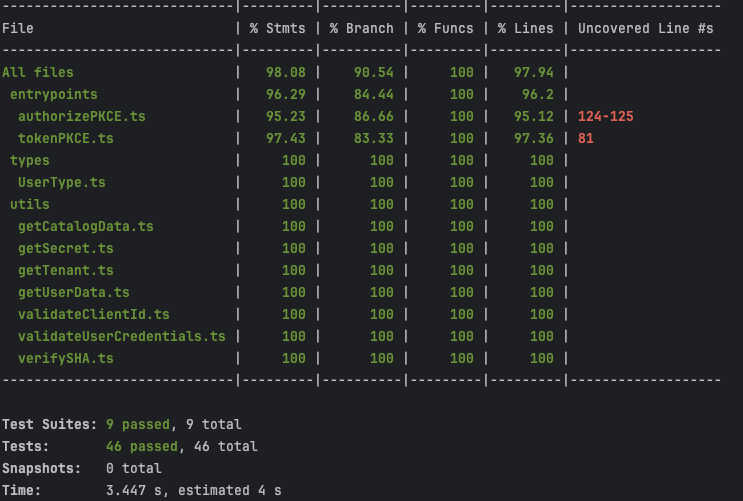
\includegraphics[width=\textwidth, height=200px]{pics/unit_test.png}} % Image with border
        \caption{Results of the Unit Test for the PKCE Prototype in Localstack}
        \label{fig:Unit Test}
    \end{figure}

    \item \textbf{Fuzz Tests:} 
    Fuzz testing was conducted by sending random or malformed input to the \textbf{/token} endpoint to identify potential vulnerabilities, such as crashes, unexpected behaviour, or unhandled exceptions. This helps ensure the endpoint is resilient to invalid or malicious inputs.

    \item \textbf{Security Scans:}
    Security scans were employed to identify potential vulnerabilities and maintain best practices:
    \begin{itemize}
        \item \textbf{Code Linting with ESLint:} 
        ESLint was utilised to identify code smells and ensure the codebase adhered to clean coding principles and established security best practices. Linting is crucial in minimizing the risk of introducing vulnerabilities by enforcing consistent code quality. The eslint-plugin-security-node plugin was used to enhance this process, which proved to be highly effective in detecting common security issues and code smells. Its integration ensured a more robust and secure codebase by proactively addressing potential weaknesses. Figure \ref{fig:lint_results} depicts the results of some code smells detected using the linter. 

                \begin{figure}[!htbp]
                     \centering
                     {\setlength{\fboxrule}{2pt} % Border thickness
                     \setlength{\fboxsep}{1pt}  % Space between image and border
                     \fbox{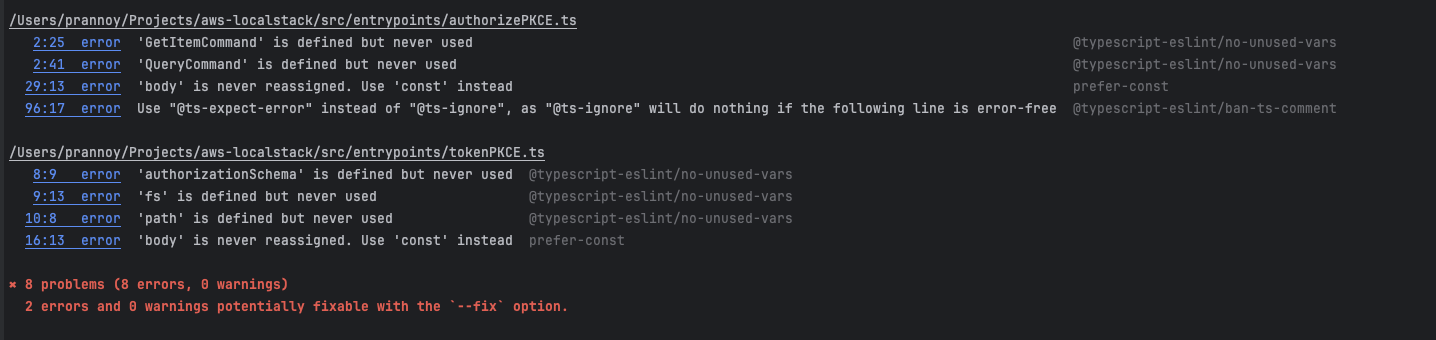
\includegraphics[width=\textwidth, height=180px]{pics/linting.png}} % Image with border
                    \caption{Lint results}
                    \label{fig:lint_results}
                \end{figure}


        \item \textbf{Cloud Infrastructure Scanning with Prowler:} 
        Prowler is a versatile open-source tool designed to scan cloud providers like AWS, helping identify potential misconfigurations in cloud infrastructure. It provides critical insights into security risks, such as overly permissive IAM roles, improper or missing logging configurations, and inadequate encryption settings. One of the critical strengths of Prowler is its ability to not only detect these issues but also provide actionable recommendations and remedies to address the identified misconfigurations. For example, as shown in Figure \ref{fig:prowler_results}, the tool detected 14 medium-level misconfigurations, each accompanied by specific remediation steps to mitigate the associated risks.

                \begin{figure}[!htbp]
                     \centering
                     {\setlength{\fboxrule}{2pt} % Border thickness
                     \setlength{\fboxsep}{1pt}  % Space between image and border
                     \fbox{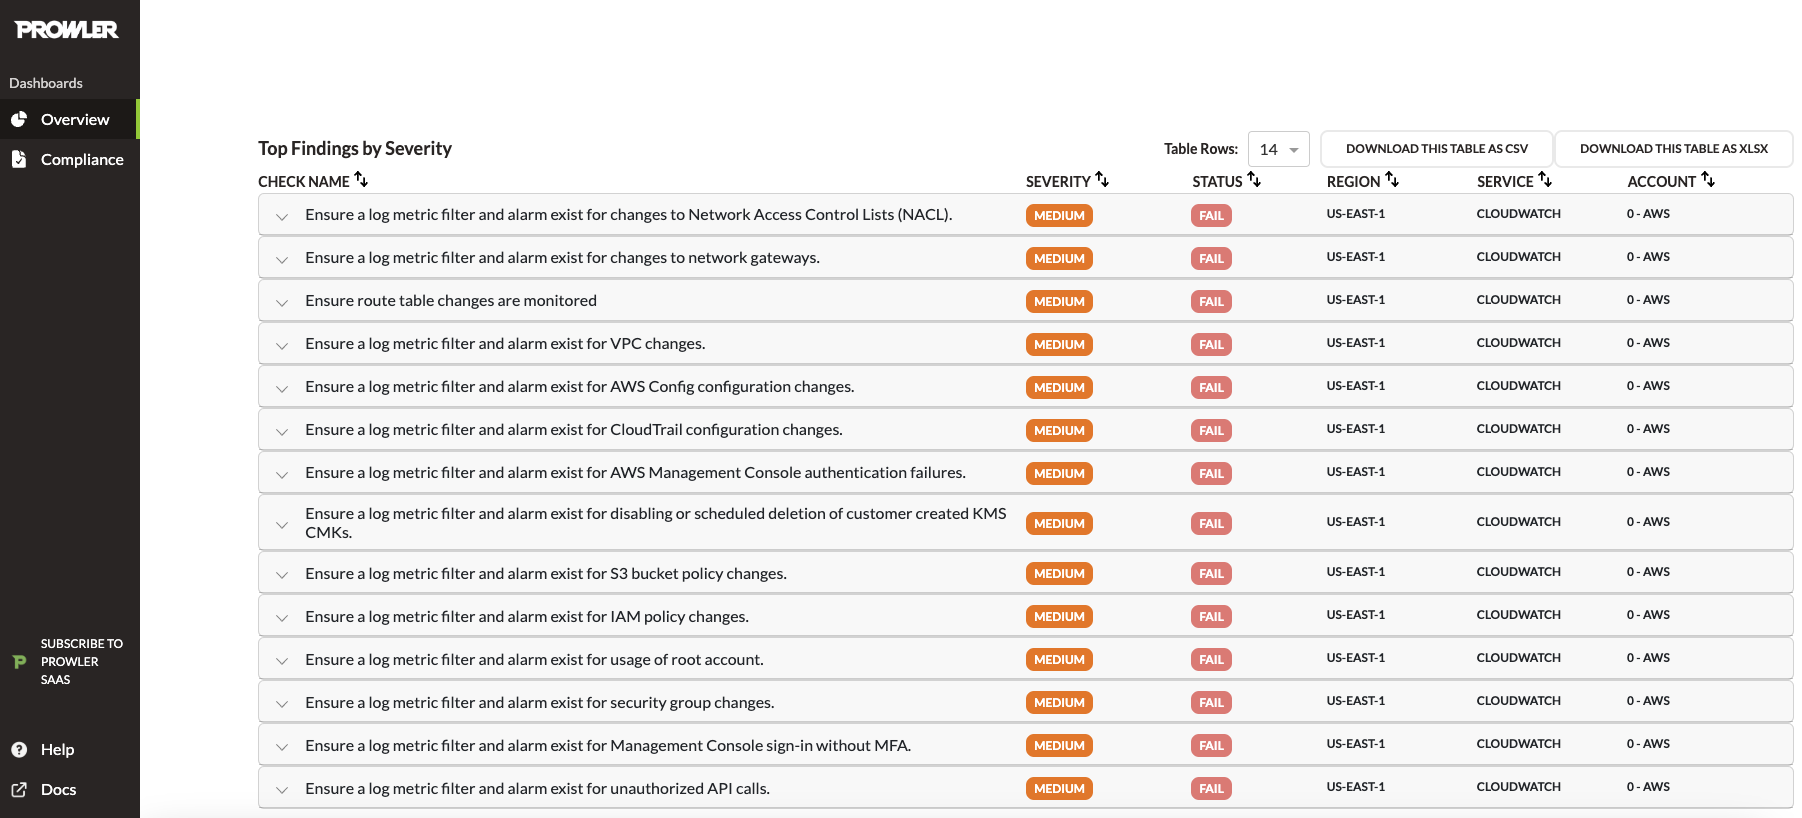
\includegraphics[width=\textwidth, height=120px]{pics/prowler.png}} % Image with border
                    \caption{Prowler Scan result}
                    \label{fig:prowler_results}
                \end{figure}

        
        In addition to the standard security checks, Prowler extends its functionality to compliance auditing. It supports testing against various industry standards, offering organisations a way to assess and strengthen their compliance posture. In this context, Prowler was utilised to perform both cloud infrastructure scans and compliance checks for ISO 27001:2013 (refer to Figure \ref{fig:prowler_iso_results}) and GDPR (refer to Figure \ref{fig:prowler_gdpr_results}). These compliance scans are particularly valuable for organisations that adhere to regulatory requirements or maintain certifications, as they provide a comprehensive view of potential gaps and actionable insights for achieving compliance.
        
                \begin{figure}[!htbp]
                     \centering
                     {\setlength{\fboxrule}{2pt} % Border thickness
                     \setlength{\fboxsep}{1pt}  % Space between image and border
                     \fbox{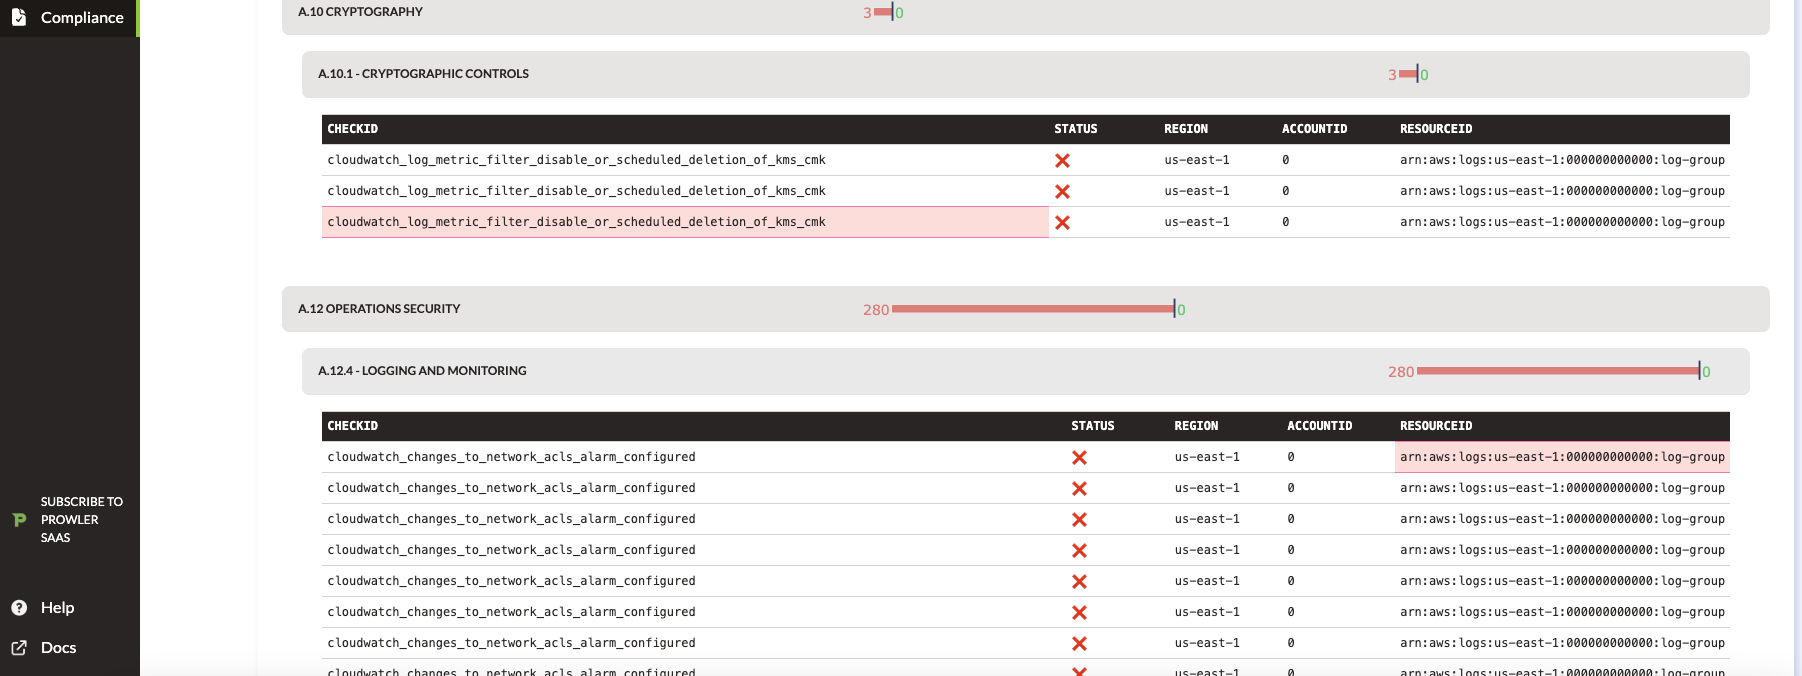
\includegraphics[width=\textwidth, height=150px]{pics/prowler_iso.png}} % Image with border
                    \caption{Prowler ISO:27001:2013 Scan result}
                    \label{fig:prowler_iso_results}
                \end{figure}

                \begin{figure}[!htbp]
                     \centering
                     {\setlength{\fboxrule}{2pt} % Border thickness
                     \setlength{\fboxsep}{1pt}  % Space between image and border
                     \fbox{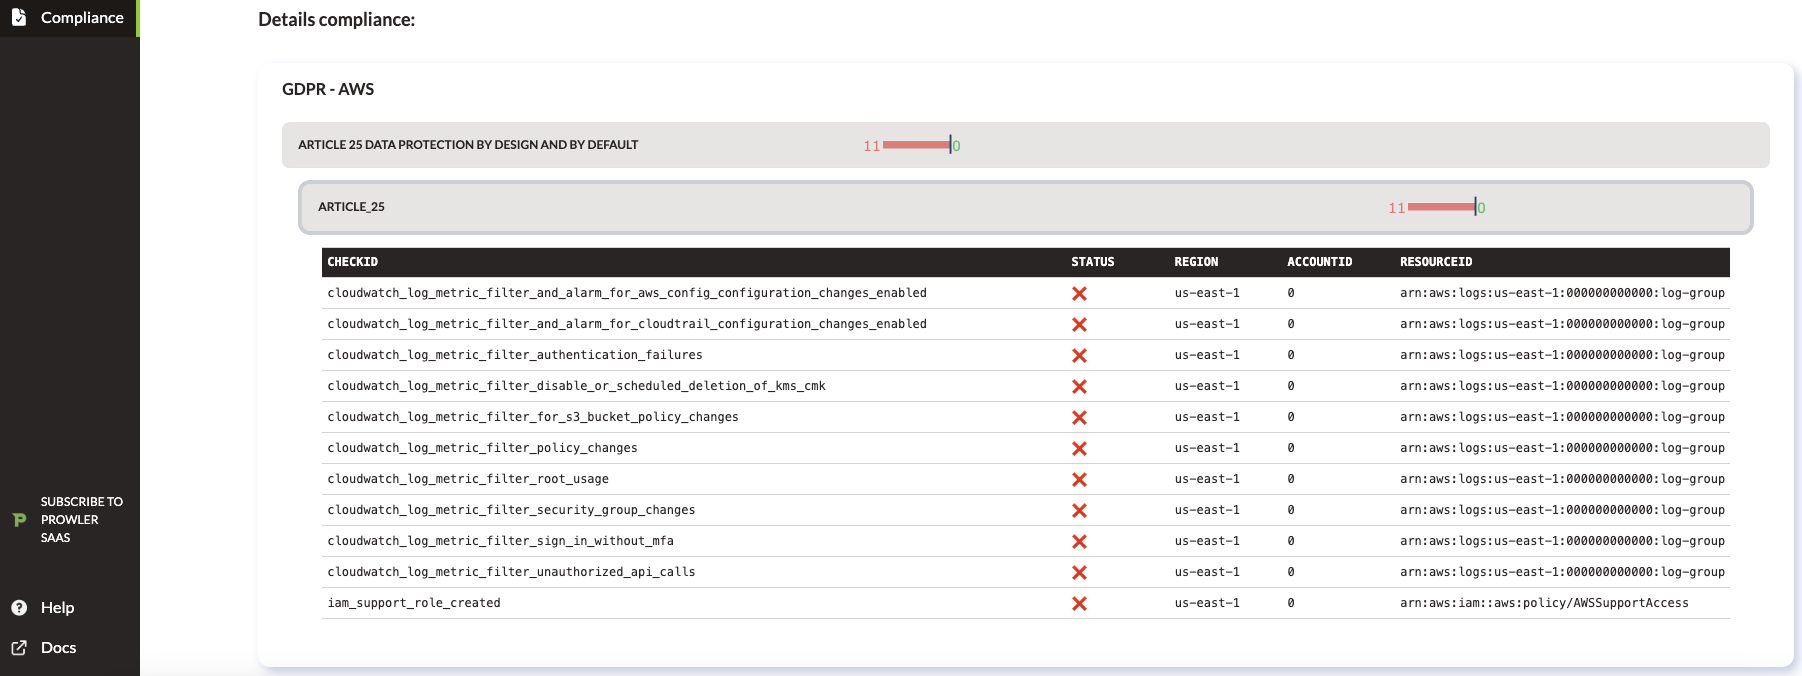
\includegraphics[width=\textwidth, height=150px]{pics/prowler_gpdr.png}} % Image with border
                    \caption{Prowler GDPR Scan result}
                    \label{fig:prowler_gdpr_results}
                \end{figure}
        By integrating security scanning with compliance testing, Prowler is a powerful tool for proactively securing cloud environments and aligning with best practices.        
    \end{itemize}
    \item \textbf{Static Code Analysis with Snyk:} Snyk is utilised in this project as a static analysis tool to detect vulnerabilities, improve code quality, and ensure secure development practices. It complements \texttt{ESLint} by focusing on security flaws in business logic and Infrastructure-as-Code (IaC). While \texttt{ESLint} enforces coding standards and detects bugs in JavaScript, Snyk extends the scope by scanning for vulnerabilities in dependencies, IaC configurations, and container images. This integration ensures both high-quality code and robust security measures. Figure \ref{fig:snyk_results} illustrates the results of Snyk's analysis.
    

    \begin{figure}[!htbp]
                     \centering
                     {\setlength{\fboxrule}{2pt} % Border thickness
                     \setlength{\fboxsep}{1pt}  % Space between image and border
                     \fbox{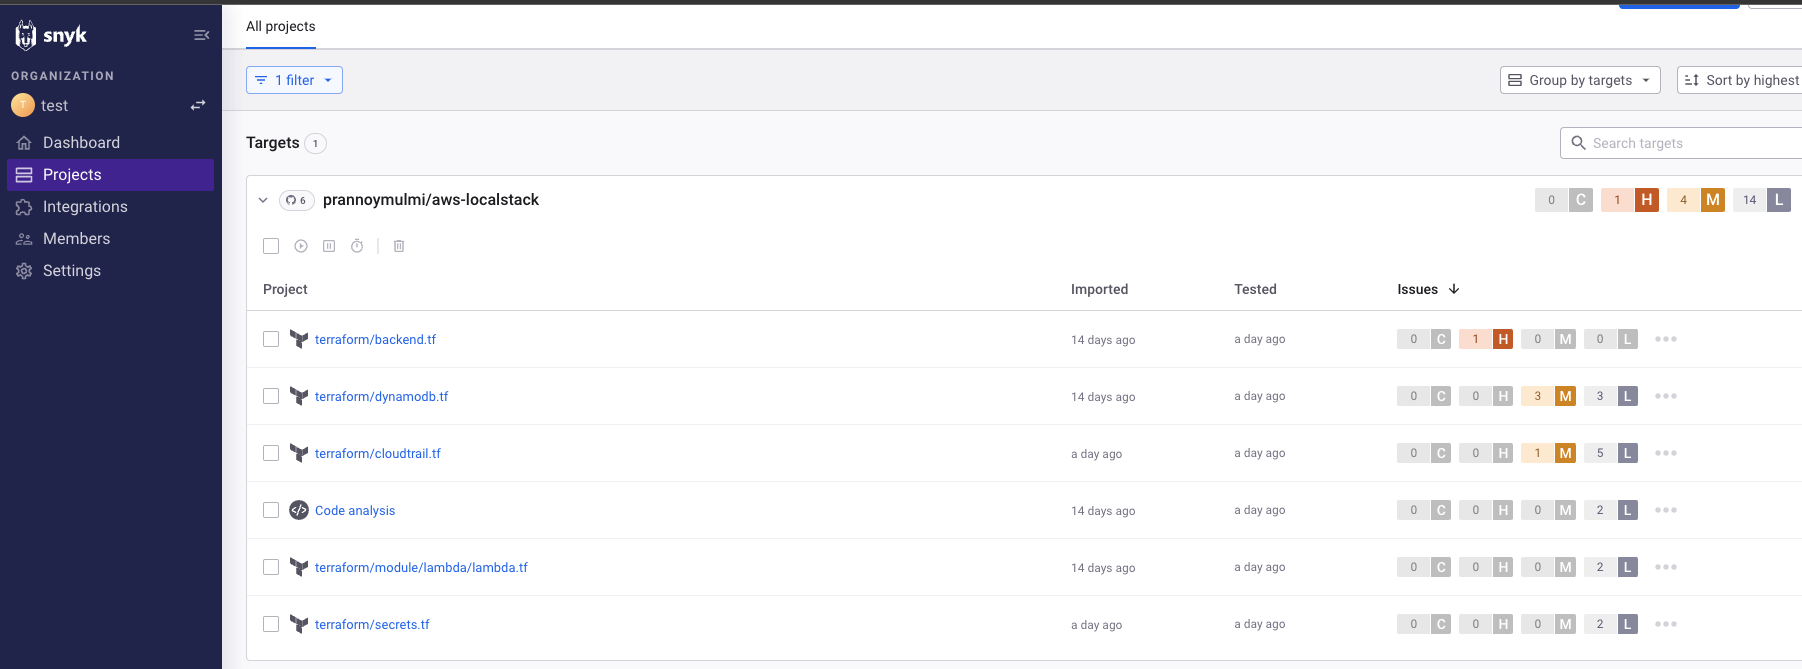
\includegraphics[width=\textwidth]{pics/snyk.png}} % Image with border
                    \caption{Static Code Analysis with Snyk}
                    \label{fig:snyk_results}
                \end{figure}
\end{enumerate}

\newpage
\section{Test Summary}
\begin{longtable}{|p{5cm}|p{10cm}|}
\hline
\rowcolor{grey!15}
\textbf{Threat} & \textbf{Test} \\
\hline
\endhead
\hline
\endfoot
Cloud Misconfigurations &  Figures \ref{fig:prowler_results} and \ref{fig:snyk_results} presents test results from Prowler and Snyk that identify several cloud misconfigurations. These tools revealed various configuration improvements that could threaten this application, providing valuable information. \\
\hline
Cross-Tenant Data Leakage & Integration tests were conducted using the tenant1 domain name to access user data from tenant 2. The tenant1 domain name limits the access to data only from tenant one. Listing \ref{apendix:cross_tenant_data_integ_test} shows the tests using the client ID of tenant two and using user credentials that belong to tenant 1. These tests both resulted in a denial of the request.\\
\hline
Code Injection (XSS, SQLi) \& Code Vulnerabilities & \begin{itemize}
    \item Unit tests were carried out where inputs of length less than 43 and more than 128 were provided. These tests rejected the requests that stood outside this range. For the implementation code, refer to Appendix \ref{apendix:rfc7636_test}.
    \item Fuzz test that inputs various random strings to detect unusual behaviour of the system. Refer to Appendix \ref{apendix:fuzz_test} to see the implementation of the fuzz tests that use different random inputs on the authorise endpoint.
\end{itemize}\\
\hline
 Unauthorised Access & Manual testing, and unit testing have been conducted where using expired authorisation code, invalid credentials, use of invalid client\_id, and invalid code\_verifier has been tested. During all the tests, access was denied, and neither the authorisation code nor the access token was issued. Refer to the Manual Testing Section \ref{subsec:auth_failure_tests} to see the results for denied access for the mentioned cases.\\
\hline
PKCE Downgrade Attack & To test the PKCE Downgrade attack, a manual authorisation request was created without a code\_challenge. During this test, the authorisation server rejected all the requests without hashed code\_challenge or missing code\_verifier. Refer to Figure \ref{fig:authorize_tenant_1_without_code_challenge} where a PKCE Downgrade attack without code\_challenge was executed.\\
\hline
Timing Attacks & A test recording the compute time to verify 1000 samples of wrong passwords and 1000 samples of correct passwords were recorded. A Pearson’s $X^{2}$ test was then performed to assess leakage detection with the two sample sets. Refer to Section \ref{sec:timing_test} for the statistical test performed and the results.\\
\hline
\end{longtable}

\section{Results} 

\subsection{Cloud Configuration: A Top Security Concern}

In this analysis, the misconfiguration of cloud services emerged as one of the most significant issues. This finding was supported by vulnerability scans conducted using \textbf{Prowler} and \textbf{Snyk}, which identified multiple configuration-related warnings and vulnerabilities across the actively used cloud services: \textbf{Amazon DynamoDB}, \textbf{Amazon API Gateway (APIGW)}, and \textbf{AWS Lambda}.

\paragraph{Security Scan Results}
\begin{itemize}
    \item \textbf{Prowler}: Prowler flagged \textbf{14 medium-severity warnings} and \textbf{1 high-severity warning} within the scanned cloud configurations. These issues highlight potential risks that could expose the environment to unauthorised access or reduce its resilience to attacks.
    \item \textbf{Snyk}: Snyk detected \textbf{1 high-severity issue}, \textbf{4 medium-severity vulnerabilities}, and \textbf{1 low-severity issue}. These findings further corroborate the need for a robust approach to managing cloud configuration risks.
\end{itemize}

\paragraph{Complexity and Scaling Risks}:
The scans were conducted for only three actively used AWS services: \textbf{DynamoDB}, \textbf{APIGW}, and \textbf{Lambda}, which represent a subset of a typical cloud environment. Despite the limited scope, the results already highlight significant concerns about misconfiguration. As the number of services grows and their interdependencies increase, the complexity of managing cloud configurations will scale significantly. This growth will likely lead to an even greater risk of misconfigurations, amplifying the potential attack surface.

Following the finding, it is necessary to emphasize that \textbf{cloud configurations represent a critical security threat}. This aligns with the assessment outlined in \ref{table:threat_model_assets}, where misconfiguration was identified as one of the top-ranked threats to the cloud environment. Misconfigured resources can lead to data breaches, service disruptions, and compliance violations, underscoring the importance of proactive configuration management and continuous monitoring.

\newpage
\subsection{Security Tools: Useful but Not Sufficient}

Security tools such as \textbf{Prowler} and \textbf{Snyk} provide valuable insights into potential vulnerabilities and misconfigurations within cloud environments. However, while these tools are effective for identifying numerous issues, they cannot be solely relied upon for ensuring a secure setup. Several limitations and shortcomings were observed during the analysis, highlighting the importance of complementing automated tools with reviews from an expert and adherence to security best practices.

\paragraph{Undetected Security Issues}

Despite their advantages, the tools failed to detect certain critical issues deliberately introduced into the environment for testing purposes. These include:

\begin{itemize}
    \item \textbf{IAM Policy Not Following the Principle of Least Privilege}: 
    A deliberately misconfigured IAM policy that violated the principle of least privilege (refer to Listing \ref{lst:bad_policy_iam}) was created as part of the test. Such a policy, if accessed by a malicious actor, could be exploited to gain elevated privileges and compromise the environment. However, this misconfiguration or bad practice was not flagged by any of the tools used in this study.

    \begin{lstlisting}[caption={Added a Bad IAM Policy that allows all actions}, label={lst:bad_policy_iam}]
# IAM Policy for Lambda to log to CloudWatch
resource "aws_iam_policy" "test_bad_policy" {
  name        = "bad policy"
  description = "IAM policy test for bad example"

  policy = jsonencode({
    Version = "2012-10-17",
    Statement = [
      {
        Effect = "Allow",
        Action = [
          "*:*"
        ],
        Resource = "*"
      }
    ]
  })
}
\end{lstlisting} 

\item \textbf{False Positives and Contextual Irrelevance}: Besides undetected issues, the tools occasionally generated \textbf{false positives} or flagged findings irrelevant to the specific use case. For instance, Prowler flagged the absence of a \texttt{support\_role} as a medium-severity issue. However, no support role was required for the use case tested, and this finding was irrelevant. Such false positives can create unnecessary noise in the results. An increase of noise in such tools could train teams to treat warnings from the tools as noise, and this could lead to an overlook of critical issues.
\end{itemize}

\subsection{Threats in OIDC and Cloud Integration}
Several well-documented threats, such as token-related risks, replay attacks, and phishing, remain critical to access in OIDC as they pose significant risks if not taken care of. Furthermore, these threats become even more significant when integrated with cloud environments, where additional complexities arise.

The complexities increase as many cloud providers offer vast services like databases, networking solutions, and application hosting. This flexibility increases the chance of choosing the wrong service and requires good knowledge of the different services. A poorly informed choice of infrastructure or security settings can inadvertently expose sensitive data, including Personally Identifiable Information (PII), to unauthorised access.

These scenarios can have severe consequences, including data leaks and regulatory violations. For example, mismanagement of access controls or insecure handling of tokens in cloud services could lead to unauthorised access. Such vulnerabilities compromise data protection and violate the regulatory framework. Namely, GDPR Article 25 and GDPR Article 32 (Refer to Section \ref{section:gdpr}) mandate "data protection by design and by default," emphasizing the importance of embedding robust safeguards into systems from the outset and proper security measures that should be taken to protect sensitive data. The risks associated with OIDC-specific and cloud-specific vulnerabilities highlight the need for heightened oversight to prevent breaches and ensure compliance with legal and regulatory standards.


      
\chapter{Conclusion}

This thesis analyses the security risks associated with implementing and using the OIDC protocol in cloud-based applications. Using a structured methodology, including threat modelling, risk assessment, and prototype development, the investigation has highlighted vital vulnerabilities and proposed mitigation strategies to enhance the security of OIDC in cloud environments.

The findings emphasise that OIDC is a robust and widely adopted protocol for authentication and authorisation. However, its security is highly dependent on proper implementation, configuration, and best practices. Several critical risks were identified, including replay attacks, signature manipulation, malicious endpoint exploitation, and PKCE downgrade attacks. Moreover, the shared responsibility model inherent to cloud computing introduces additional challenges, such as misconfigurations in Identity and Access Management (IAM) policies.

Security testing further demonstrated that cloud misconfigurations remain a significant concern. Whereas automated security testing tools such as Prowler and Snyk are valuable for identifying vulnerabilities, they are insufficient without expert review and adherence to best practices. Even with well-established protocols and cloud providers, OIDC and AWS, respectively, meticulous knowledge and the right choice of tools are key to reducing vulnerabilities.   


\section{Future Work}

\begin{itemize} 
    
    \item Although this study mainly focused on user-based tokens and their associated security risks within the OpenID Connect (OIDC) protocol, it is essential to note that OIDC also supports machine-to-machine (M2M) communication, also known as client authentication \citep{openid_docs}. In M2M scenarios, client authentication is crucial, as it involves server-to-server interactions without human intervention. More research on the security risks of M2M communication, especially with cloud integration, would be beneficial in complementing the findings of this study.

    \item Enhancing cyber hygiene and reducing cloud misconfigurations are critical for future exploration. Addressing cloud misconfigurations resulting from human error or oversight can significantly reduce the risk of unauthorised access and data breaches. A study that could provide effective measures against misconfigurations can significantly benefit sensitive data security.

    \item The prototype contains some limitations, as the cloud environment was simulated using a local stack.
    Some real-world scenarios could not be tested.
    For example, testing the domain name resolution to set specific headers to identify tenants was impossible.
    Also, local machines cannot cope with more load like the cloud, making it untested for a real-life scenario and its scalability.
    By leveraging AWS's infrastructure, one can test features like auto-scaling and multi-region deployments under actual conditions, offering more accurate insights into performance and scalability.
    Although deploying on AWS incurs costs, it enables comprehensive testing with real-world data, ensuring that the application can handle production-level demands effectively.
\end{itemize}






By expanding research into these areas, organisations can better secure their cloud environments and more effectively leverage OIDC for user-based and machine-to-machine communications.




% ---- Bibliography ----
%
% BibTeX users should specify bibliography style 
% References will then be sorted and formatted in the correct style.
%
 %\bibliographystyle{alpha}
\renewcommand{\bibname}{References}
\bibliographystyle{agsm}
\bibliography{biblio}
\appendix
\chapter{Tool Results}


\lstdefinestyle{bashstyle}{
    language=bash,
    basicstyle=\ttfamily\small, % Monospaced font, smaller size
    backgroundcolor=\color{lightgray}, % Light gray background
    frame=single, % Frame around the code block
    numbers=left, % Line numbers on the left
    numberstyle=\tiny\color{gray}, % Style for line numbers
    keywordstyle=\color{blue}, % Color for keywords
    commentstyle=\color{green}, % Color for comments
    stringstyle=\color{red}, % Color for strings
}
\appendix
\chapter{Setup}
\begin{lstlisting}[style=bashstyle,caption=Build and run script,label=apendix:build_and_run_script]
#! /bin/bash

BUCKET_NAME="state-bucket"
FIRST_RUN=true  # Set FIRST_RUN as a boolean (without quotes)
VOLUME_DIR="./volume"
RUN_ALL=false
RUN_DB=false

# Check for --run-all flag
for arg in "$@"; do
  if [ "$arg" == "--run-all" ]; then
    RUN_ALL=true
    break
  fi
done

# Check for --run-all flag
for arg in "$@"; do
  if [ "$arg" == "--run-db" ]; then
    RUN_DB=true
    break
  fi
done

if [ ! -d "$VOLUME_DIR" ]; then
  mkdir -p "$VOLUME_DIR"
  echo "Directory '$VOLUME_DIR' created."
fi

# Check if the bucket exists
if ! awslocal s3api head-bucket --bucket "$BUCKET_NAME" 2>/dev/null; then
    # Create the bucket if it doesn't exist
    echo "Bucket does not exist, creating it..."
    awslocal s3api create-bucket --bucket "$BUCKET_NAME"
    echo "Bucket '$BUCKET_NAME' created."
else
    echo "Bucket '$BUCKET_NAME' already exists."
    FIRST_RUN=false  # Update the boolean
fi

yarn clean
yarn install
#yarn build
yarn deploy

# Define the target directory
tf_dir="./terraform"

# Run commands inside the target directory without changing the current directory
if ! $RUN_DB; then
  (
    cd "$tf_dir" || exit
    pwd
    rm -rf .terraform
    tflocal init
    tflocal apply -auto-approve
  )
fi
# Check if it's the first run
if $FIRST_RUN || $RUN_ALL || $RUN_DB; then
  # Add this at the top of your script to import the argon2 library
  node -e "require('argon2');"

  # Function to hash passwords using Argon2id
  hash_password() {
    local PASSWORD="$1"
    node -e "
      const argon2 = require('argon2');
      argon2.hash('$PASSWORD', { type: argon2.argon2id }).then(hash => console.log(hash)).catch(err => console.error(err));
    "
  }

  for k in {1..2}
  do
    awslocal dynamodb put-item \
                --table-name "catalog-table" \
                --item "{
                    \"tenantId\": {\"S\": \"tenant$k\"},
                     \"table_name\": {\"S\": \"tenant-$k-table\"},
                     \"client_ids\": {\"L\": [{\"S\": \"tenant$k-client-id-1\"}, {\"S\": \"tenant$k-client-id-2\"}, {\"S\": \"tenant$k-client-id-3\"}]}
                }"
    echo "Inserted tenant$k in catalog-table"
    for i in {1..10}
      do
        # Generate a random userId and email
        userId="user-$RANDOM-$RANDOM"
        email="user$i@example.com"
        password="test$k"
        hashed_password=$(hash_password "$password")

        # Insert into DynamoDB using awslocal
        awslocal dynamodb put-item \
          --table-name "tenant-$k-table" \
          --item "{
              \"id\": {\"S\": \"$userId\"},
              \"codeChallenge\": {\"S\": \"some-code-verifier-$i\"},
              \"user_email\": {\"S\": \"$email\"},
              \"password\": {\"S\": \"$hashed_password\"},
              \"userProfile\": {
                  \"M\": {
                      \"name\": {\"S\": \"User $i\"},
                      \"email\": {\"S\": \"$email\"}
                  }
              }
          }"

        echo "Inserted user with userId $userId and email $email in tenant-$k-table"
      done
  done
fi

# Add tenant domain into local hosts file
if $FIRST_RUN; then
  # Host entries to add
  HOST1="127.0.0.1 tenant1.local"
  HOST2="127.0.0.1 tenant2.local"
  HOSTS_FILE="/etc/hosts"

  # Function to add a host entry if it doesn't exist
  add_host_if_missing() {
      local HOST_ENTRY="$1"
      local HOSTS_FILE="$2"

      if ! grep -qF "$HOST_ENTRY" "$HOSTS_FILE"; then
          echo "$HOST_ENTRY" | sudo tee -a "$HOSTS_FILE" > /dev/null
          echo "Added $HOST_ENTRY to $HOSTS_FILE"
          sudo dscacheutil -flushcache
          sudo killall -HUP mDNSResponder
      else
          echo "$HOST_ENTRY already exists in $HOSTS_FILE"
      fi
  }

  # Add tenant1.local and tenant2.local if they are missing
  add_host_if_missing "$HOST1" "$HOSTS_FILE"
  add_host_if_missing "$HOST2" "$HOSTS_FILE"
fi
\end{lstlisting}


\begin{lstlisting}[style=bashstyle,caption=Create Private Keys,label=apendix:create_private_keys]
#!/bin/bash

KEYS_DIR="terraform/keys"
PRIVATE_KEY_FILE="$KEYS_DIR/private.pem"
PUBLIC_KEY_FILE="$KEYS_DIR/public.pem"

# Create the keys directory if it doesn't exist
if [ ! -d "$KEYS_DIR" ]; then
  mkdir -p "$KEYS_DIR"
  echo "Directory '$KEYS_DIR' created."
fi

# Generate the private key if it doesn't exist
if [ ! -f "$PRIVATE_KEY_FILE" ]; then
  openssl genpkey -algorithm RSA -out "$PRIVATE_KEY_FILE" -pkeyopt rsa_keygen_bits:2048
  echo "Private key generated and saved to '$PRIVATE_KEY_FILE'."
else
  echo "Private key already exists at '$PRIVATE_KEY_FILE'."
fi

# Generate the public key if it doesn't exist
if [ ! -f "$PUBLIC_KEY_FILE" ]; then
  openssl rsa -pubout -in "$PRIVATE_KEY_FILE" -out "$PUBLIC_KEY_FILE"
  echo "Public key generated and saved to '$PUBLIC_KEY_FILE'."
else
  echo "Public key already exists at '$PUBLIC_KEY_FILE'."
fi
\end{lstlisting}
% formatting taken from http://tex.stackexchange.com/questions/149708/simple-list-of-abbreviations-manually
% sorting taken from http://www.latex-community.org/forum/viewtopic.php?f=44&t=16419

\end{document}
